%This is chapter 4
%%=========================================
\chapter{Result}
This chapter presents the results of this thesis. The chapter starts with presenting the different JavaScript projects developed and improved in connection with this thesis. First, the new three-voxel-loader three.js plugin, and the improvements of the Voxelizer engine are presented. This is followed by the new BINVOX package, and the desktop application for the Voxelizer engine. Then, the results of the JSDoc GitHub Action is presented. Section~\ref{sec:result-automation} will present the results in terms of automation of the projects. Finally, Section~\ref{sec:result-popularity-and-achievements} presents some additional achievements, including some statistics on the popularity of the projects.

\section{three-voxel-loader}
The three-voxel-loader is a plugin for three.js. It is published to the npm registry under the name "\href{https://www.npmjs.com/package/three-voxel-loader}{three-voxel-loader}", and the source code is available at GitHub under "\href{https://github.com/andstor/three-voxel-loader}{andstor/three-voxel-loader}".

The plugin is able to generate a three.js mesh based on voxel data in a variety of data formats. Figure~\ref{fig:three-voxel-loader} shows a screenshot of a VOX model loaded with the three-voxel-loader plugin.
\begin{figure}[htp]
    \centering
    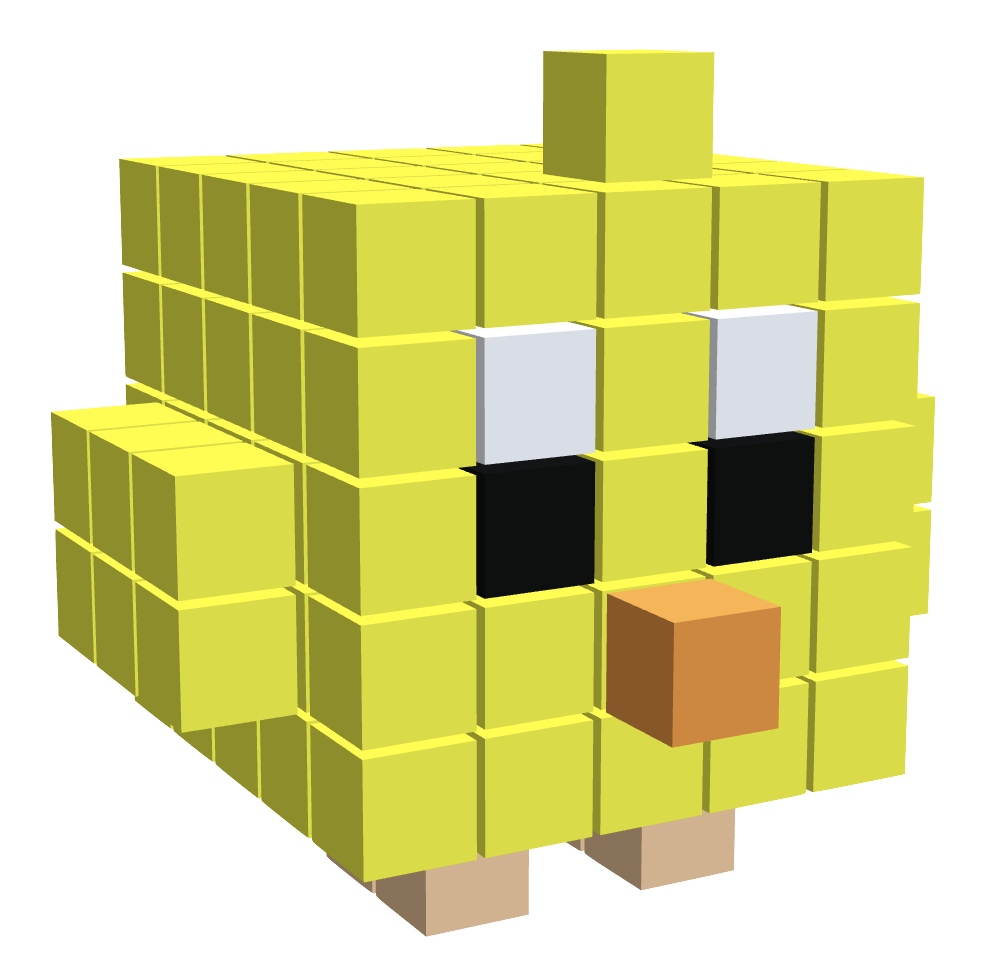
\includegraphics[width=0.45\textwidth]{sections/result/figures/chicken-voxels.png}
    \caption{Screenshot of Chicken stored in VOX file format loaded with the three-voxel-loader plugin.}
    \label{fig:three-voxel-loader}
\end{figure}
It is also possible to control the size of the individual voxels. This is shown in Figure~\ref{fig:chicken-voxels-sizes}. The size can be any number between $\left<0, 1\right]$.
\begin{figure}[htp]
    \centering
    \begin{subfigure}[t]{0.45\textwidth}
        \centering
        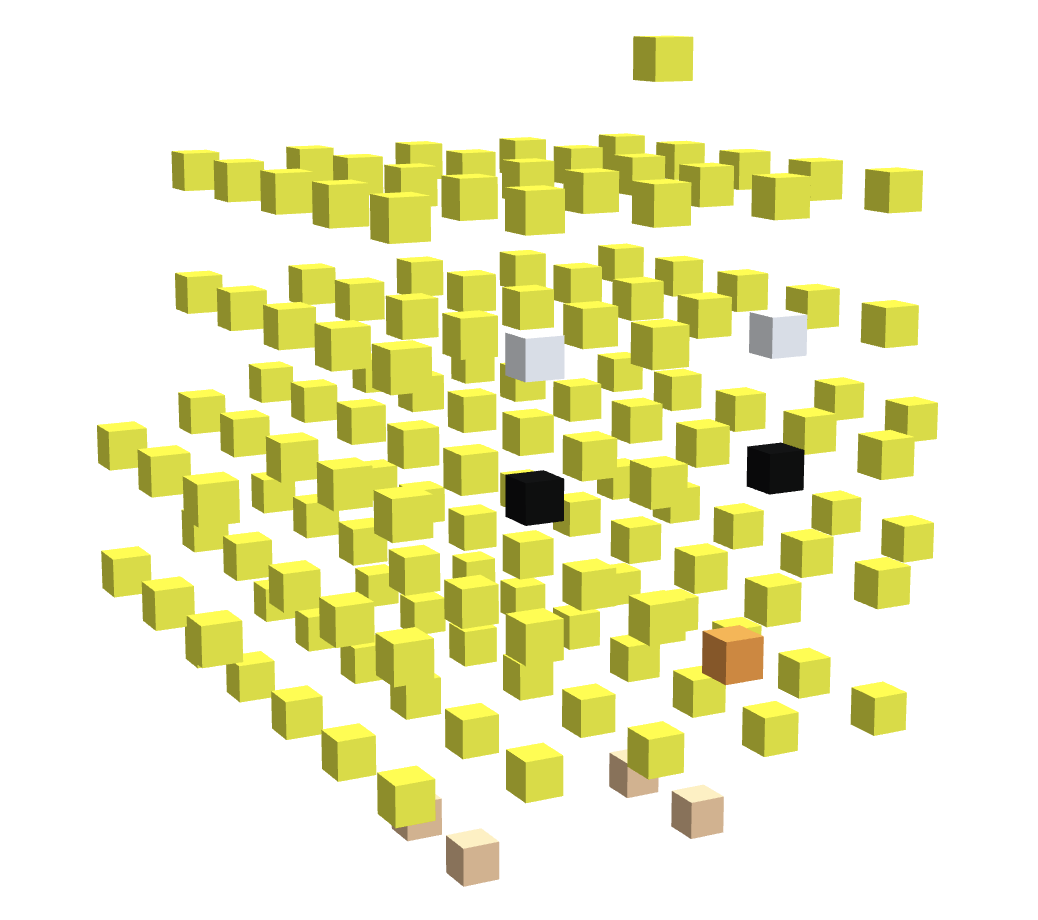
\includegraphics[width=\textwidth]{sections/result/figures/chicken-voxels-size-0.3.png}
        \caption{Voxel size set to 0.3.}
        \label{fig:chicken-voxels-size-0.3}
    \end{subfigure}
    \hfill
    \begin{subfigure}[t]{0.45\textwidth}
        \centering
        
\includegraphics[width=\textwidth]{sections/result/figures/chicken-voxels-size-1.png}
        \caption{Voxel size set to 1.}
        \label{fig:chicken-voxels-size-1}
    \end{subfigure}
       \caption{Generated meshes of different voxel sizes with the three-voxel-loader plugin.}
       \label{fig:chicken-voxels-sizes}
\end{figure}


\subsection{Level Of Detail}
The plugin implements a Level Of Detailing (LOD) system. Figure~\ref{fig:torus-lod} shows four images of a torus loaded with different LODs. Depending of the resolution of the model, a very high number of triangles may be generated. By using the LOD system, this number can be drastically reduced. For example, the mesh in Figure~\ref{fig:torus-lod-10} consists of 406,068 triangles. By setting the LOD (maxDepth) to 2, the number is reduced to only 768 triangles, still preserving the shape. This can be seen in Figure~\ref{fig:torus-lod-2}.
\begin{figure}[htp]
    \centering
    \begin{subfigure}[t]{0.45\textwidth}
        \centering
        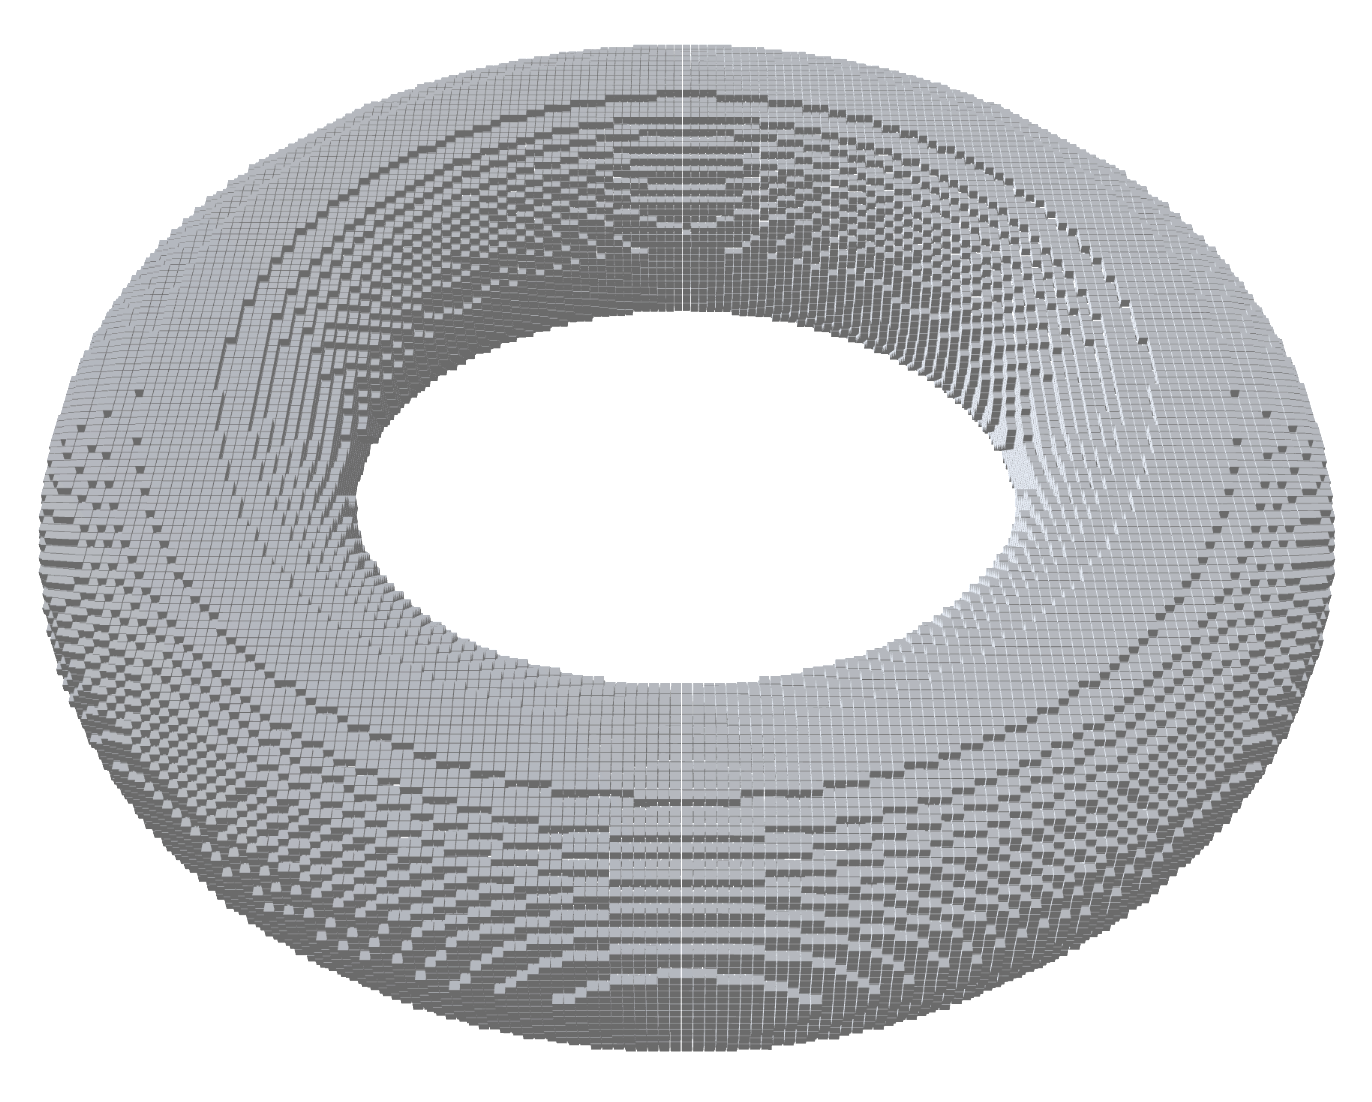
\includegraphics[width=\textwidth]{sections/result/figures/torus-lod-10.png}
        \caption{Full resolution torus mesh (406068~triangles).}
        \label{fig:torus-lod-10}
    \end{subfigure}
    \hfill
    \begin{subfigure}[t]{0.45\textwidth}
        \centering
        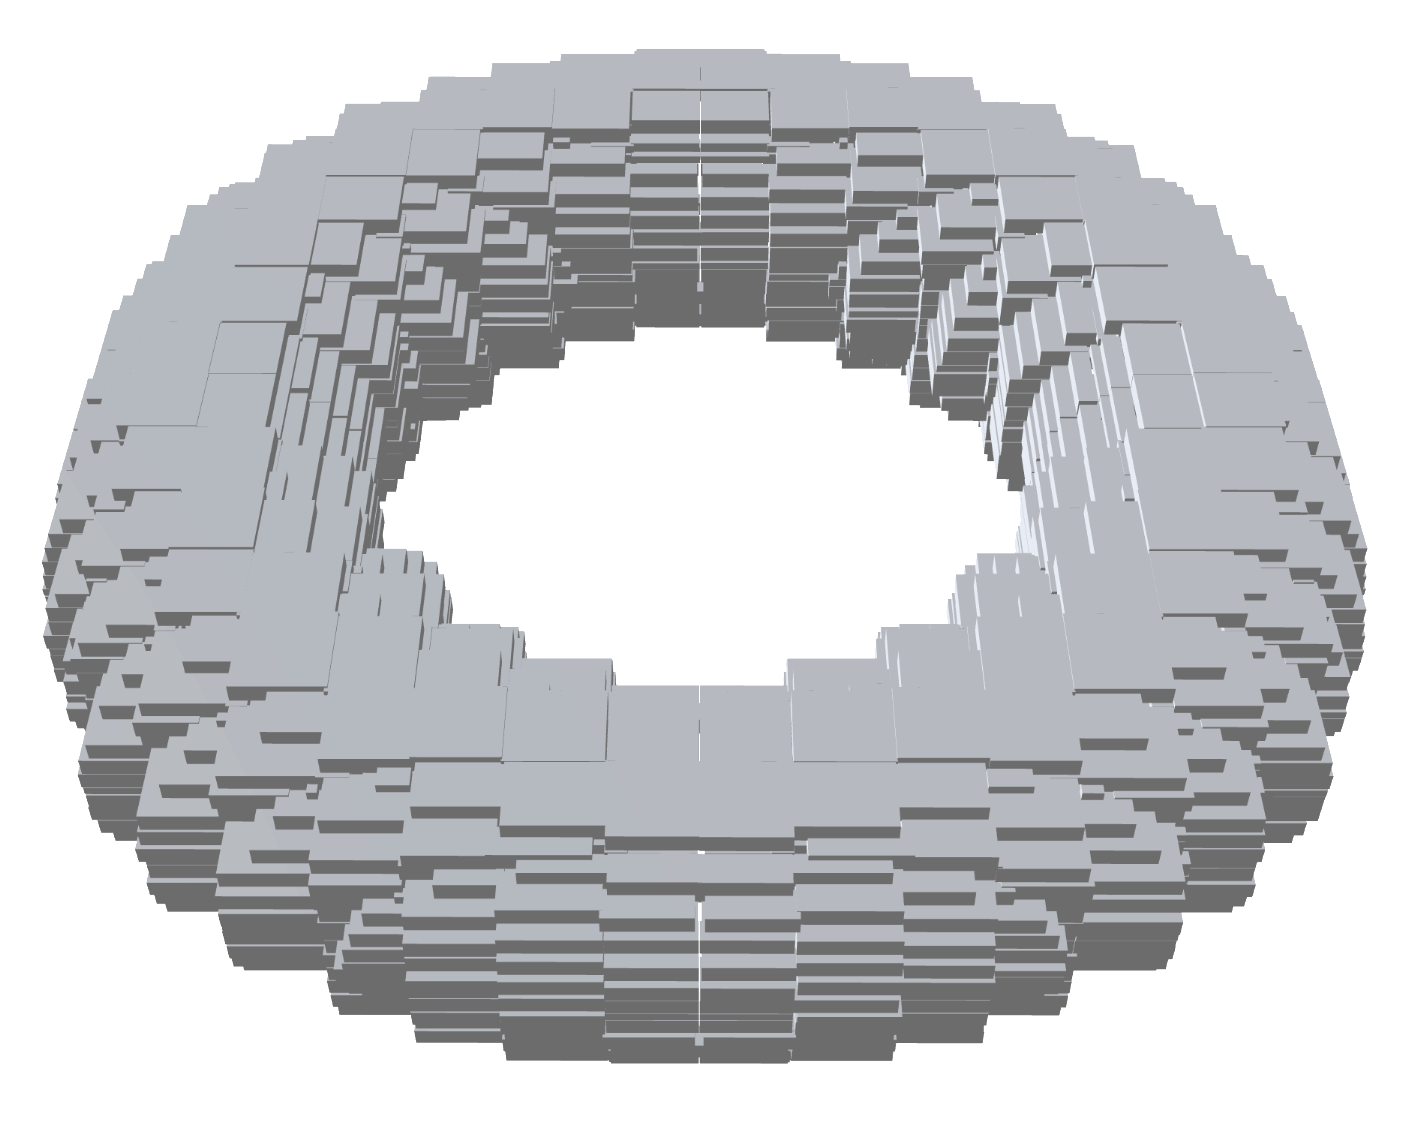
\includegraphics[width=\textwidth]{sections/result/figures/torus-lod-4.png}
        \caption{Simplified torus mesh (19740~triangles) with a LOD (maxDepth) of 4.}
        \label{fig:torus-lod-4}
    \end{subfigure}
    \hfill
    \begin{subfigure}[t]{0.45\textwidth}
        \centering
        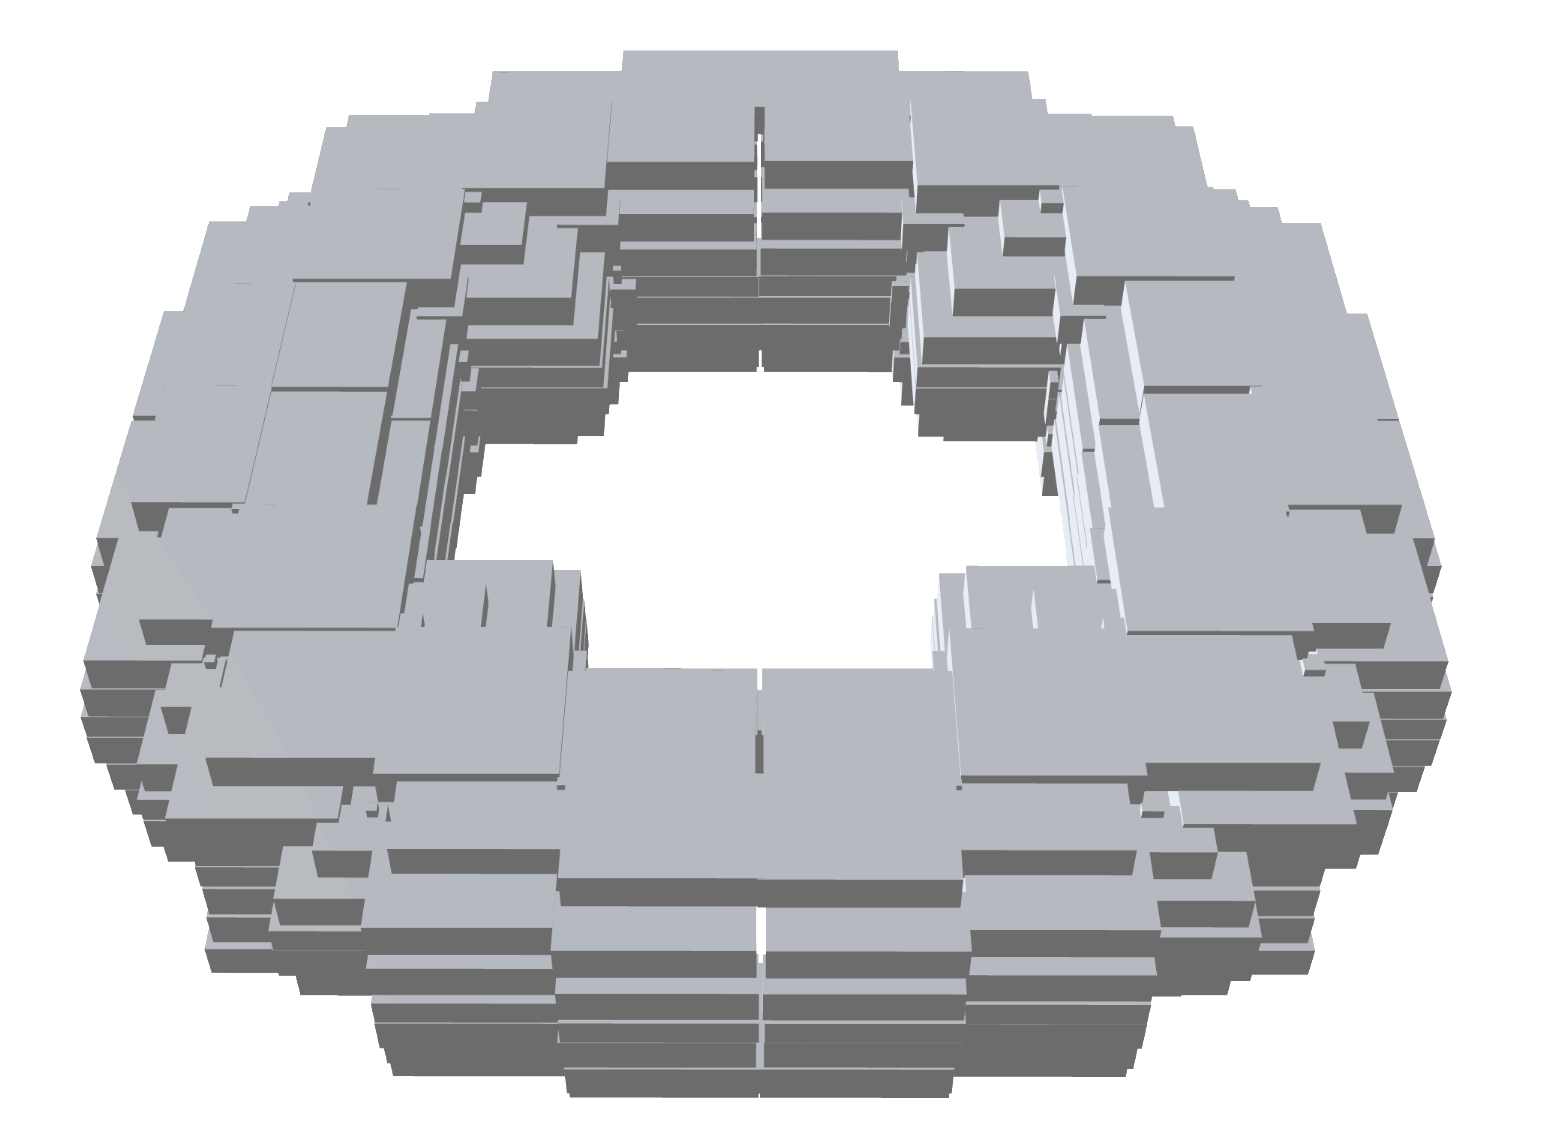
\includegraphics[width=\textwidth]{sections/result/figures/torus-lod-3.png}
        \caption{Quite simplified torus mesh (4752~triangles) with a LOD (maxDepth) of 3.}
        \label{fig:torus-lod-3}
    \end{subfigure}
    \hfill
    \begin{subfigure}[t]{0.45\textwidth}
        \centering
        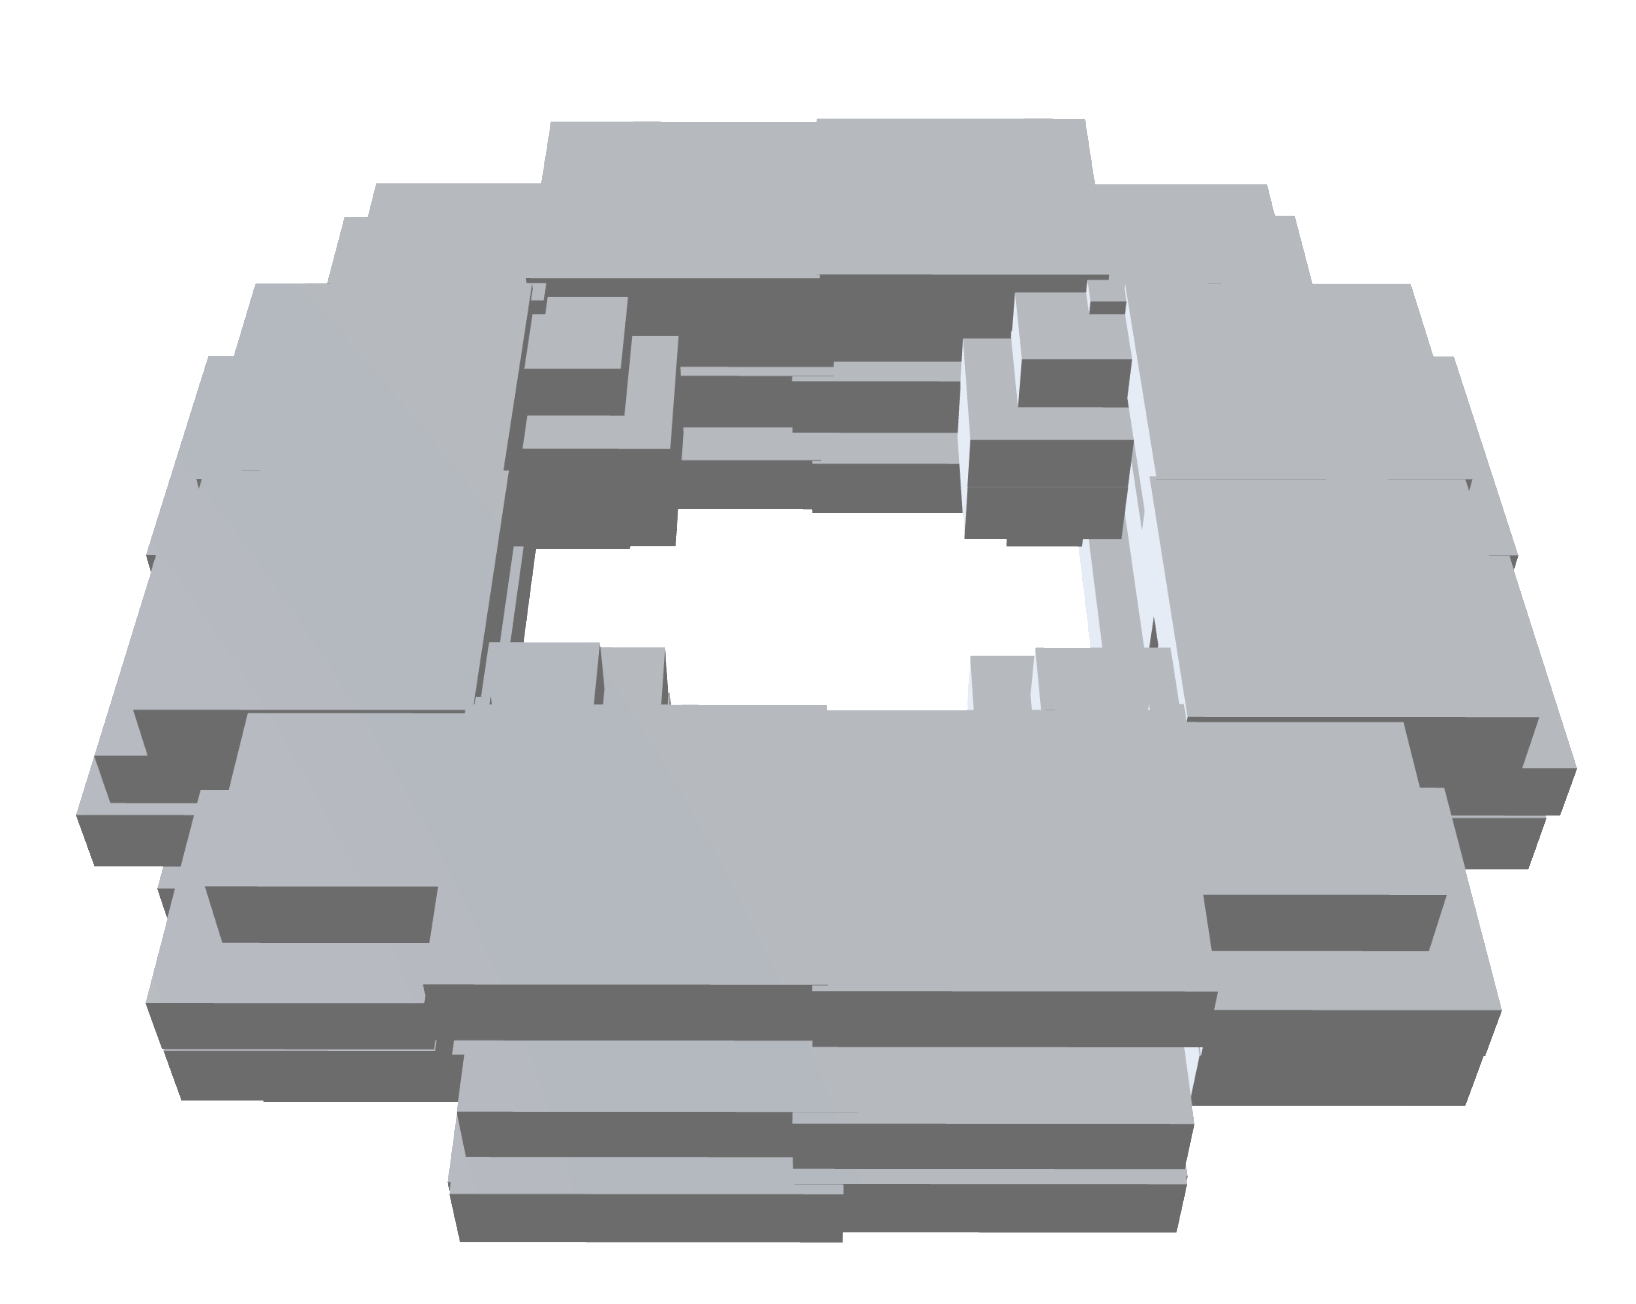
\includegraphics[width=\textwidth]{sections/result/figures/torus-lod-2.png}
        \caption{Very low detail torus mesh (768~triangles) with a LOD (maxDepth) of 2.}
        \label{fig:torus-lod-2}
    \end{subfigure}
       \caption{Torus meshes with diffrent LOD levels.}
       \label{fig:torus-lod}
\end{figure}

\subsection{Loading support}
The plugin is able to load a variety of different voxel data formats. This includes XML, VOX, BINVOX and JavaScript arrays (3D array). In addition to the raw voxel data, the three-voxel-loader plugin also supports color. The data formats that support this is XML, VOX and JavaScript arrays (4D array for color data).

\subsection{Example}
An example of the plugin is deployed to GitHub Pages. Visit \url{https://andstor.github.io/three-voxel-loader/examples/} to see the example. Figure~\ref{fig:three-voxel-loader-example} shows a screenshot of the site. The example includes a GUI with controls for changing, among other things, the voxel size and the LOD.
\begin{figure}[ht]
    \centering
    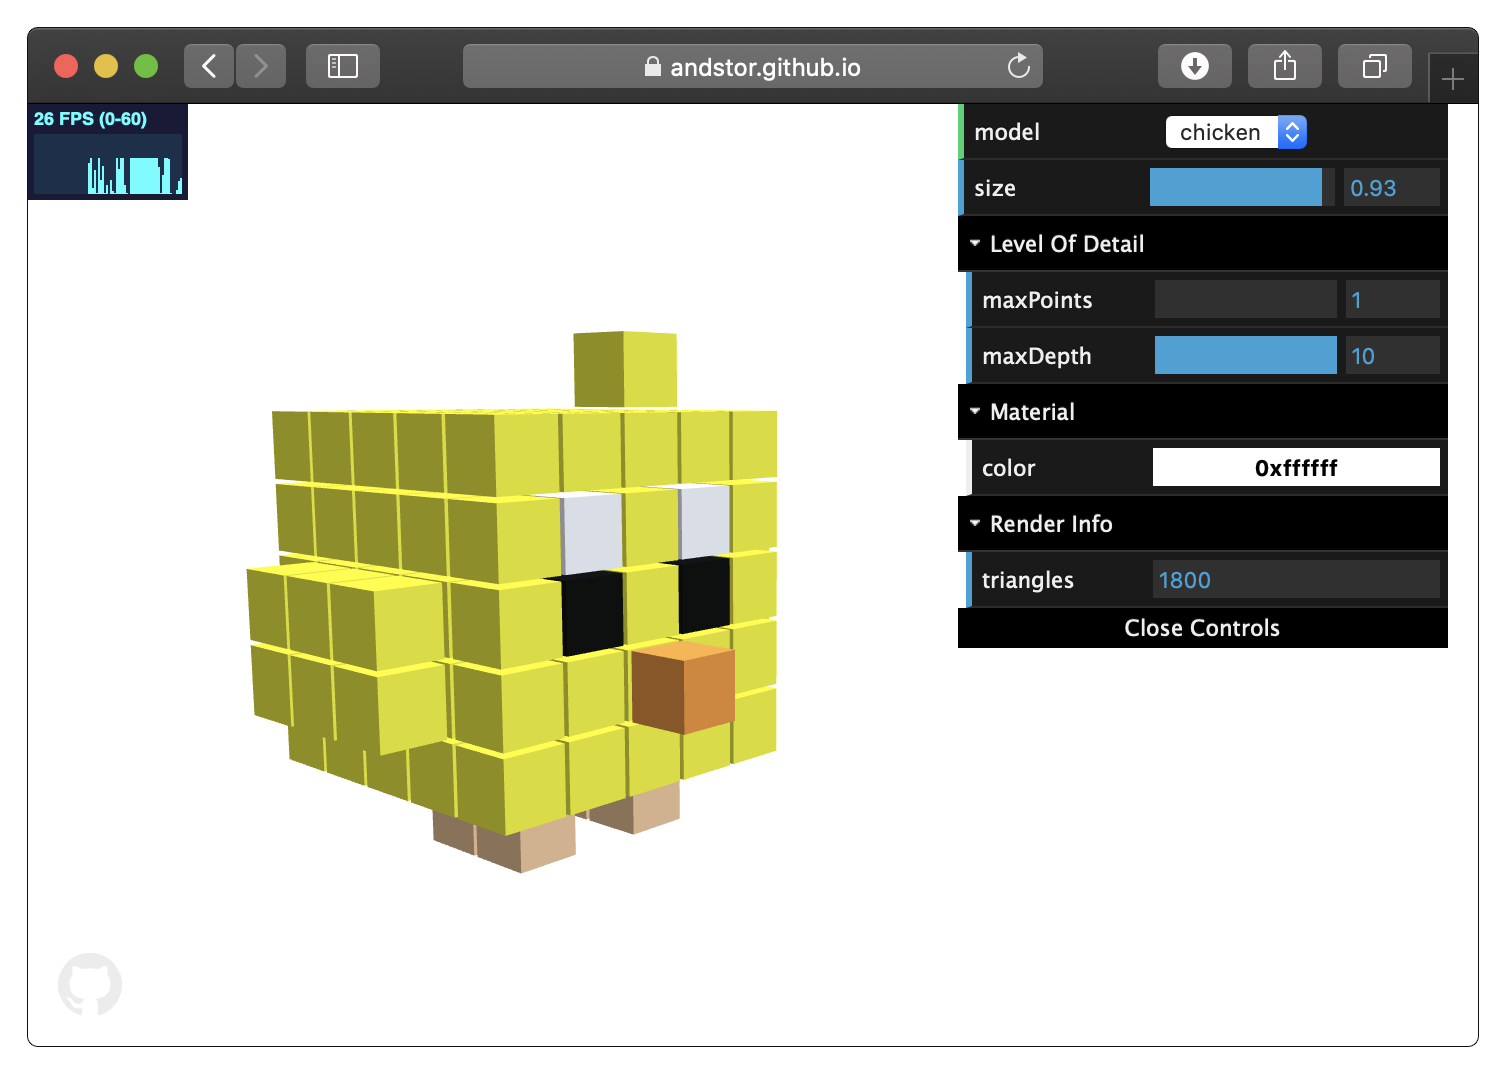
\includegraphics[width=0.9\textwidth]{sections/result/figures/three-voxel-loader-example.png}
    \caption{Screenshot of the three-voxel-loader example page at GitHub Pages.}
    \label{fig:three-voxel-loader-example}
\end{figure}

\section{Voxelizer}
The new Voxelizer engine version v1.0.0 is greatly improved, compared to the old version v0.1.3. The engine is completly redesigned, and resolves all known problems and bugs the old engine had. Further, several new features are implemented, making the engine even more powerfull. Among the new features are support for coloring and shell voxelization, in addition to several new exporting formats. The performance of the engine is also drastically improved. Other improvements includes both code quality and documentation. In order to provide the engine with an own identity, a new logo for the engine is created, as shown in Figure~\ref{fig:voxelizer-logo}.
\begin{figure}[htp]
    \centering
    
\includegraphics[width=0.5\textwidth]{sections/result/figures/voxelizer-logo.eps}
    \caption{Logo for the Voxelizer engine v1.0.0.}
    \label{fig:voxelizer-logo}
\end{figure}

The new version is published to the npm registry, still under the name "\href{https://npmjs.org/package/voxelizer}{voxelizer}". The source code is available at GitHub under "\href{https://github.com/andstor/voxelizer}{andstor/voxelizer}". Here, the old version is also available, tagged with the tag "\href{https://github.com/andstor/voxelizer/tree/v0.1.3}{v0.1.3}".

\subsection{Voxelization}
The new version of the Vexelizer engine is greatly improved. The engine captures a lot more deatils of the 3D models. It is much more stabile, and produces a lot more consistent results. The engine also provides several new voxelization features. This includes both shell voxelization, and coloring support. Figure~\ref{fig:anvil-render} shows a rendered image of an anvil 3D model developed for testing purposes. The anvil has a blue-ish metallic surface, with several red/gold rust spots. Figure~\ref{fig:result-anvil-voxelization} shows a colored voxelization of this 3D model at a resolution of $2^7$. The individual rust spots are clearly seen, and the overall result seems to be correlating with the original 3D model. Further, in order to showcase the shell voxelization, the voxelization result is cut in half. This is seen in Figure~\ref{fig:result-anvil-voxelization-cut}.
\begin{figure}[htp]
    \centering
    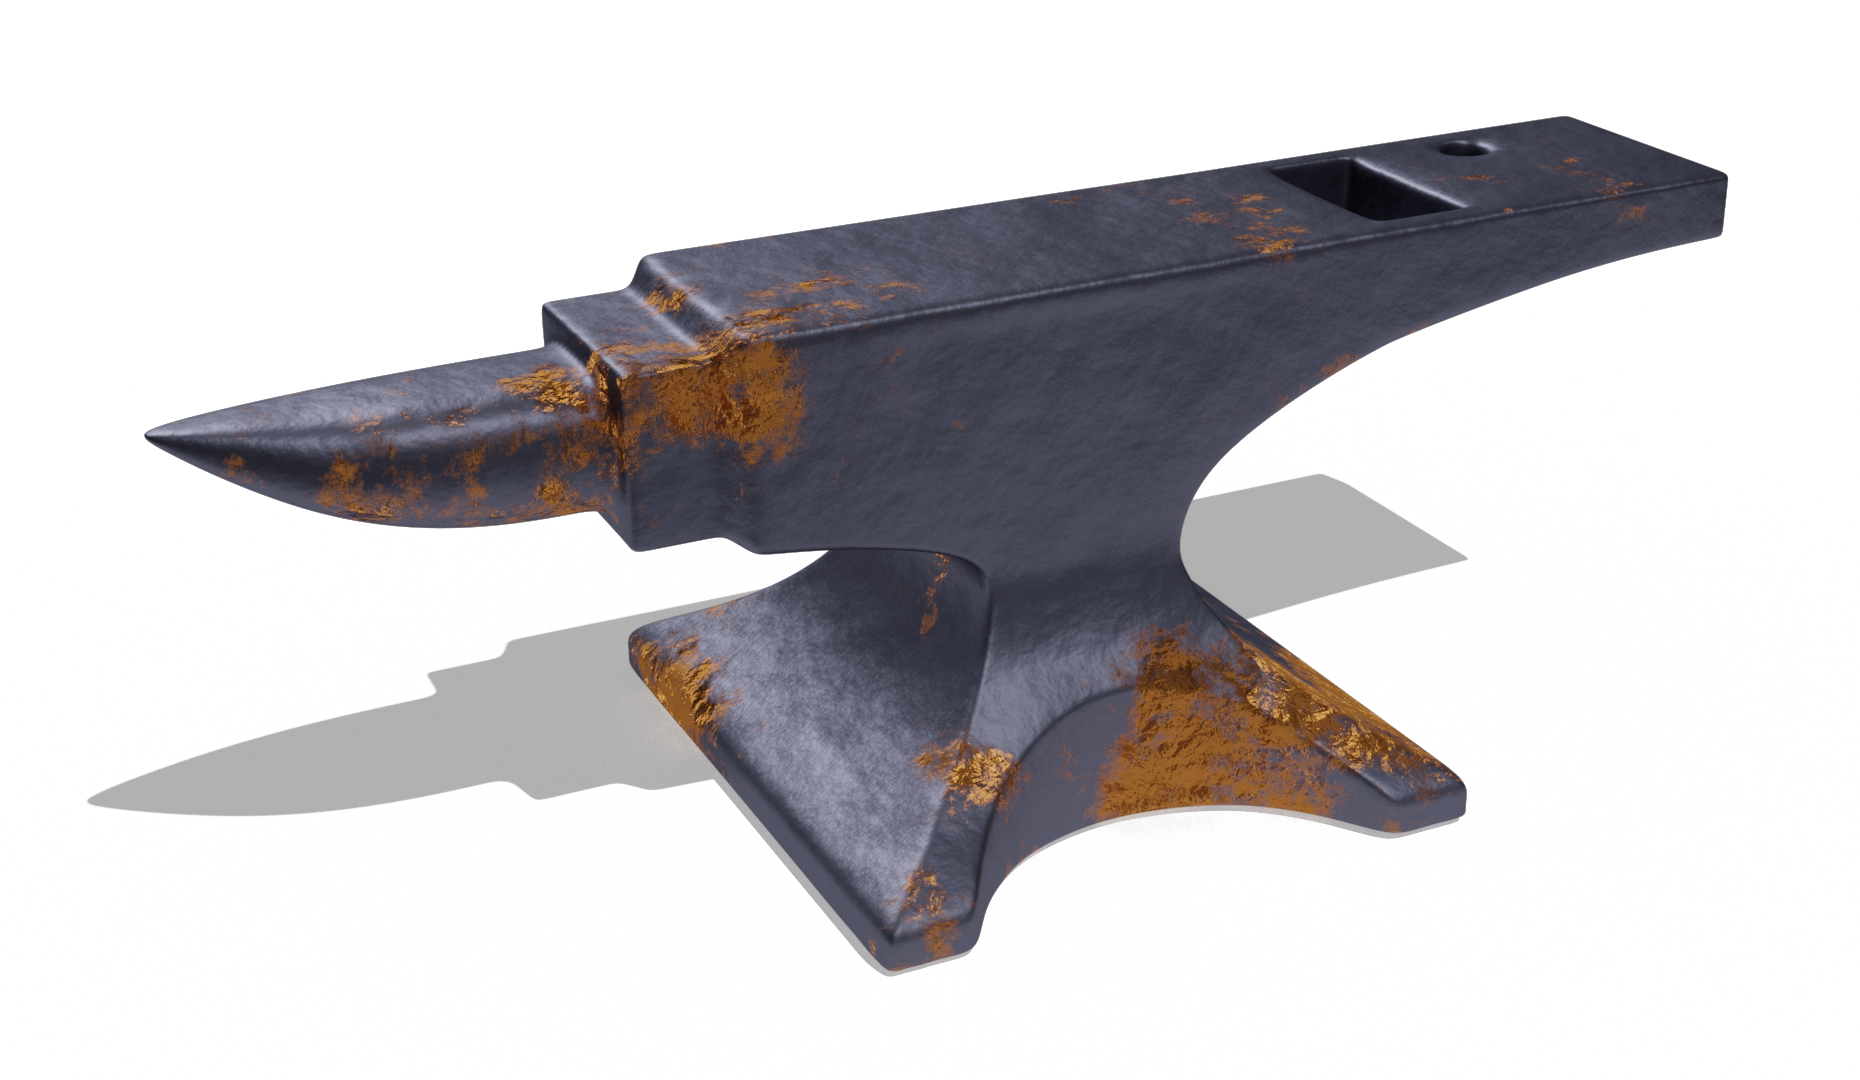
\includegraphics[width=0.95\textwidth]{sections/result/figures/anvil-color-render.png}
    \caption{Render of textured anvil 3D model.}
    \label{fig:anvil-render}
\end{figure}
\begin{figure}[htp]
    \centering
    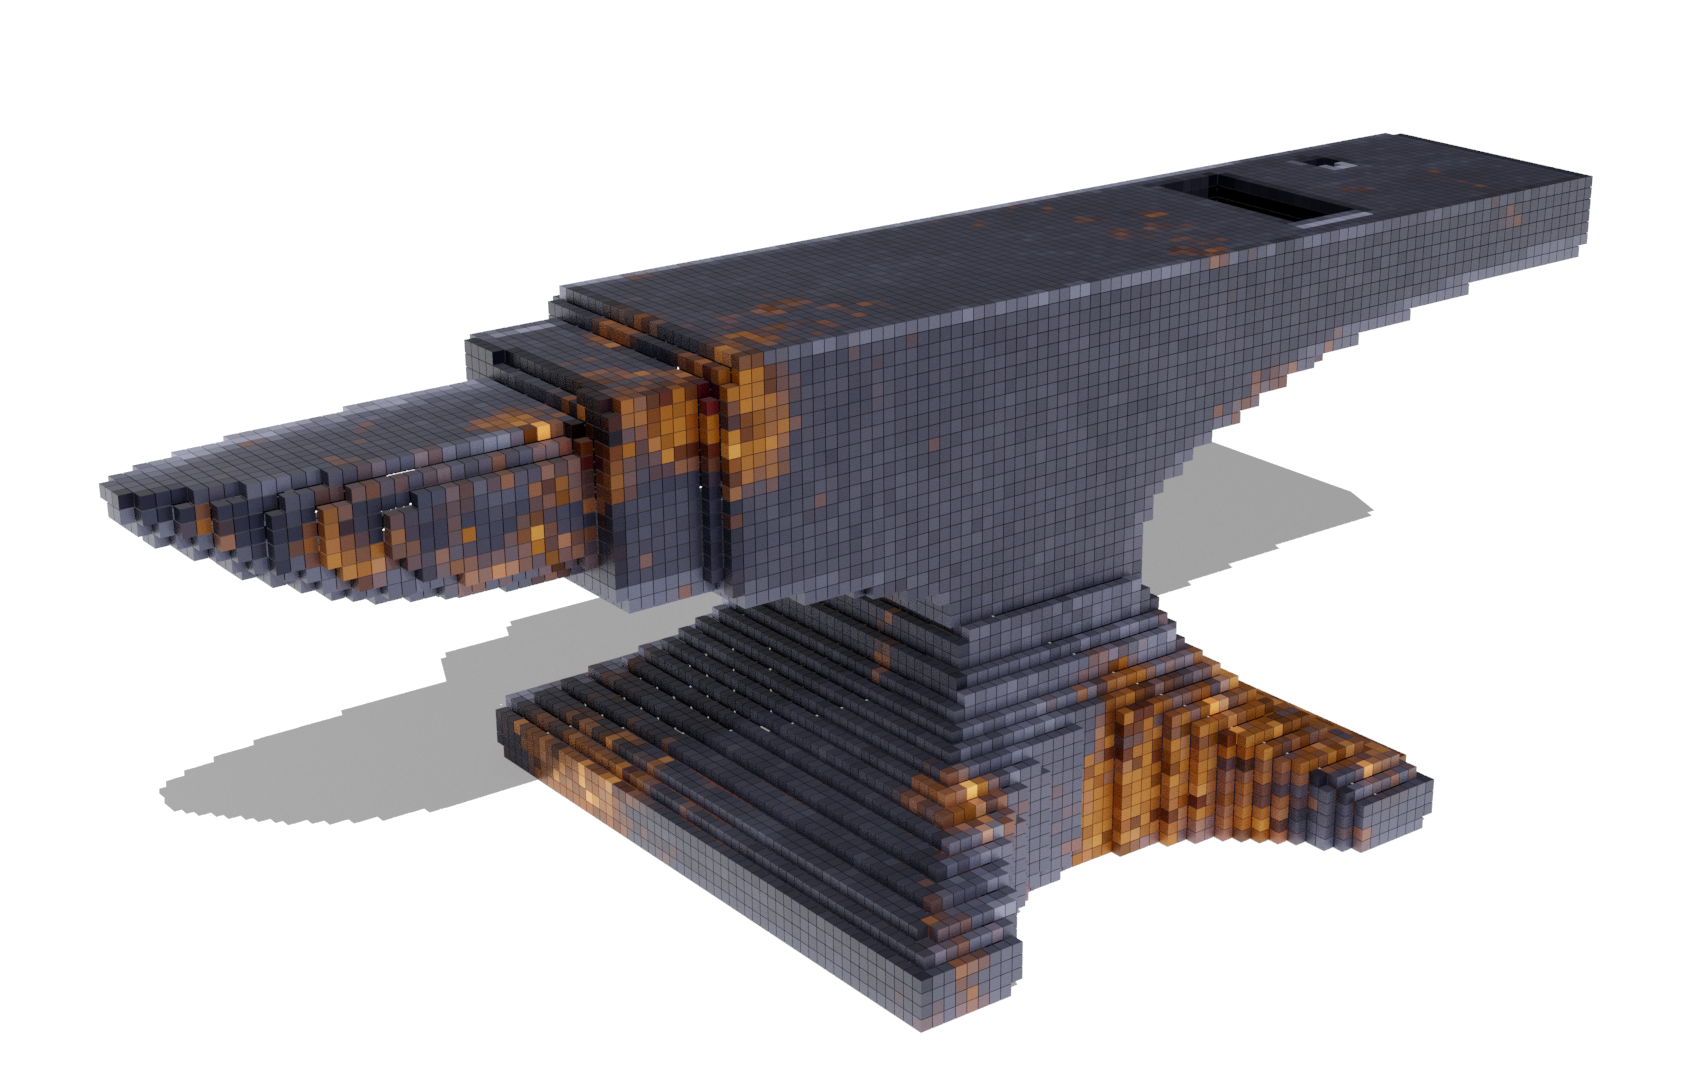
\includegraphics[width=0.95\textwidth]{sections/result/figures/anvil-voxelized-v1-color-128.png}
    \caption{Colored voxelization (resolution of $2^7$) of anvil 3D model.}
    \label{fig:result-anvil-voxelization}
\end{figure}
\begin{figure}[htp]
    \centering
    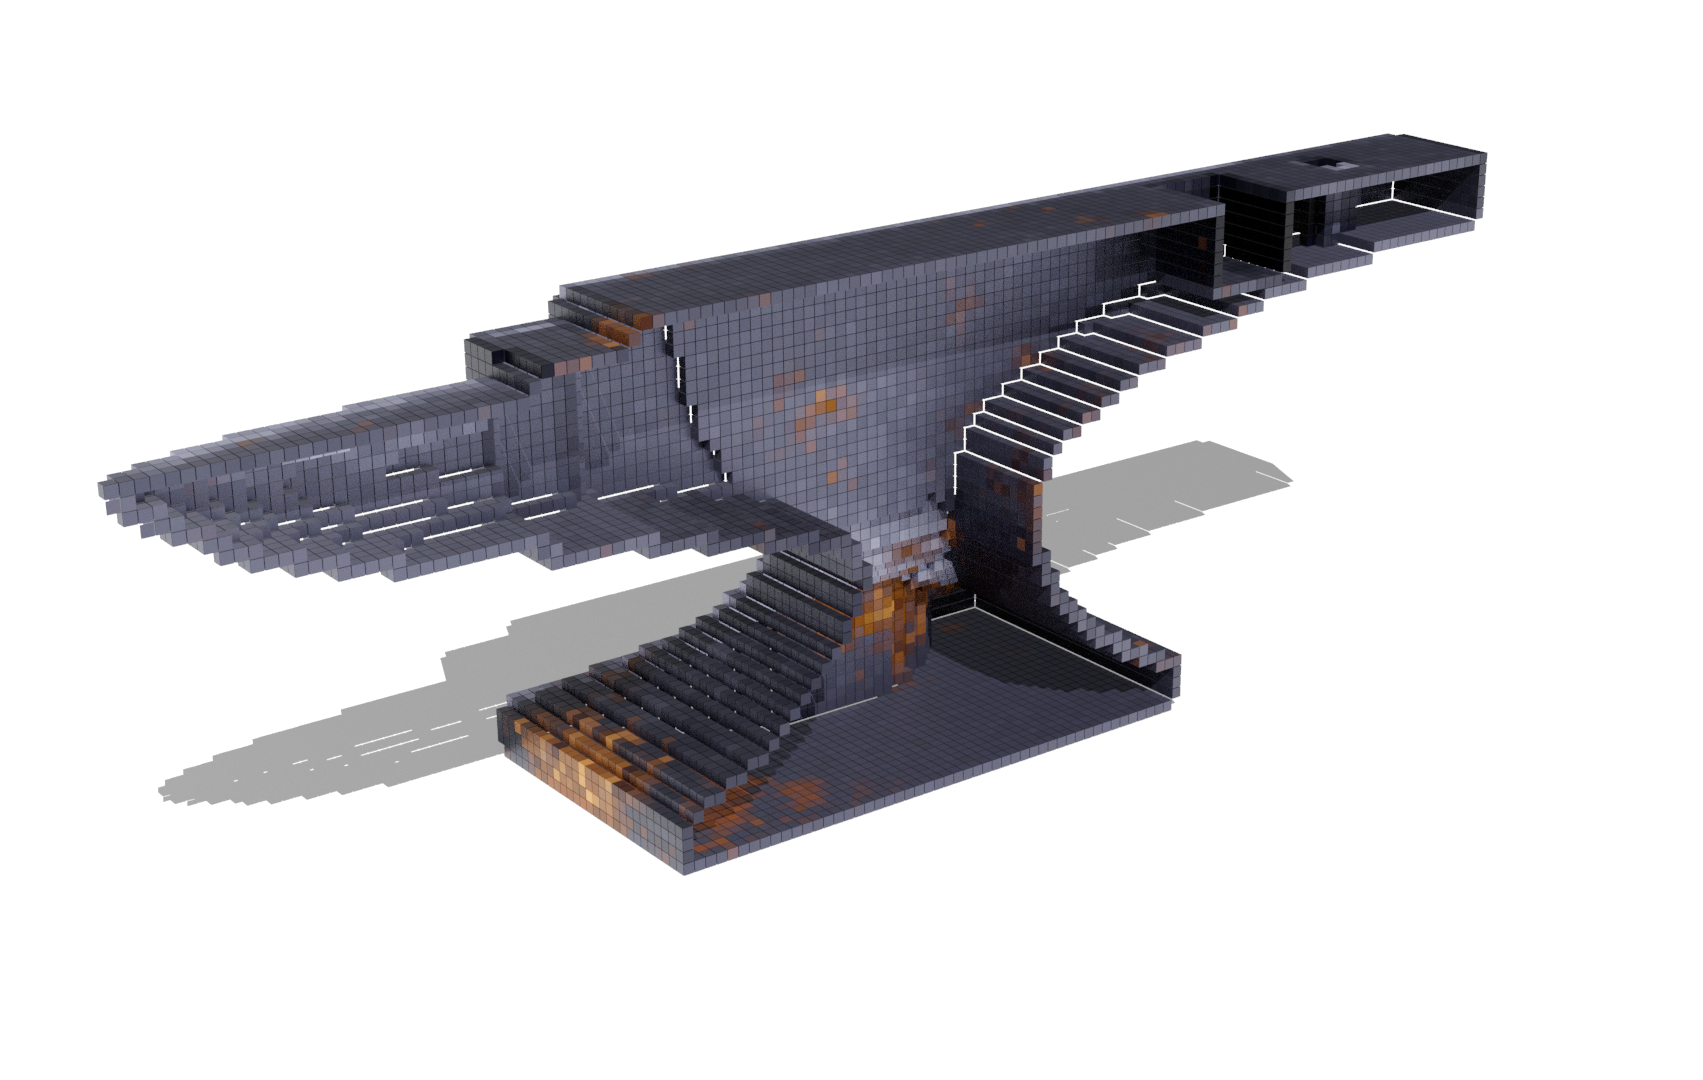
\includegraphics[width=0.95\textwidth]{sections/result/figures/anvil-voxelized-clipped-v1-color-128.png}
    \caption{Colored voxelization (resolution of $2^7$) of anvil 3D model cut in half.}
    \label{fig:result-anvil-voxelization-cut}
\end{figure}

\clearpage
\subsection{Visual assesment}
\label{sec:method-visual-assesment}
In this section, the various improvements of the problems the old engine had is presented. Fistly, the old engine produced several holes. The new version fixes this problem. This can be seen in Figure~\ref{fig:result-voxelizer-comparison-torus}, which shows the voxelization of a torus 3D model. Figure~\ref{fig:result-voxelizer-v0.1.3-torus} shows the voxelization of a torus with the old version, and Figure~\ref{fig:result-voxelizer-v1-torus} shows the result with the new version. Comparing the two, it is clear that the holes are no longer present.
\begin{figure}[htp]
    \centering
    \begin{subfigure}[b]{0.49\textwidth}
        \centering
        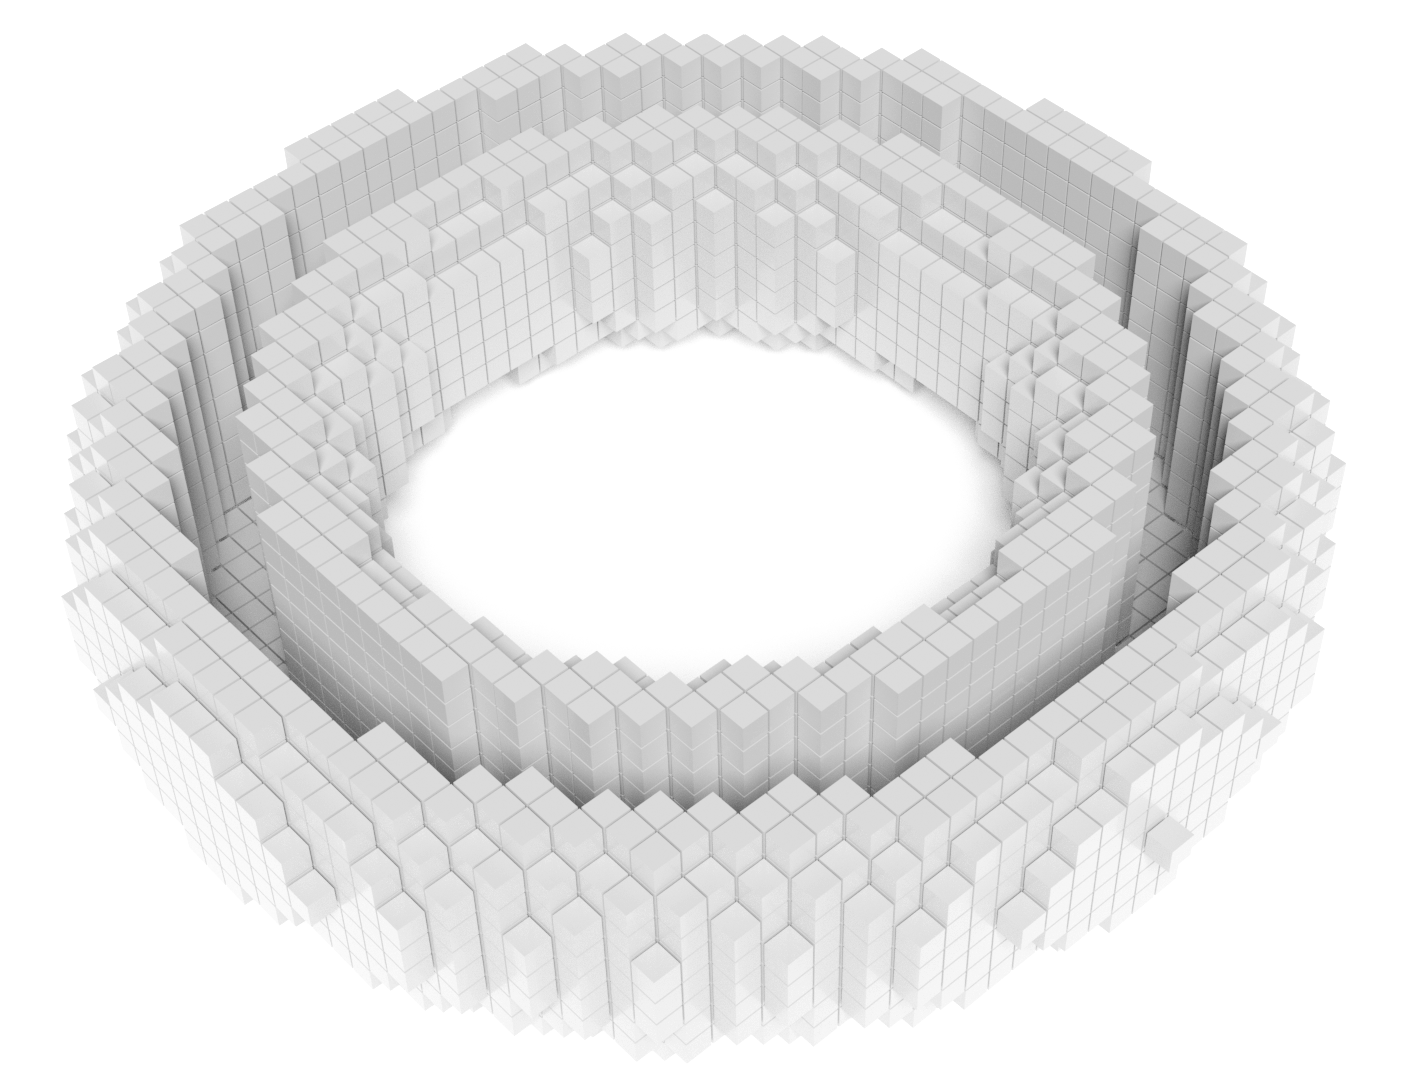
\includegraphics[width=\textwidth]{sections/theory/figures/voxelizer-v013-torus-40.png}
        \caption{Voxelized torus with Voxelizer v0.1.3.}
        \label{fig:result-voxelizer-v0.1.3-torus}
    \end{subfigure}
    \hfill
    \begin{subfigure}[b]{0.49\textwidth}
        \centering
        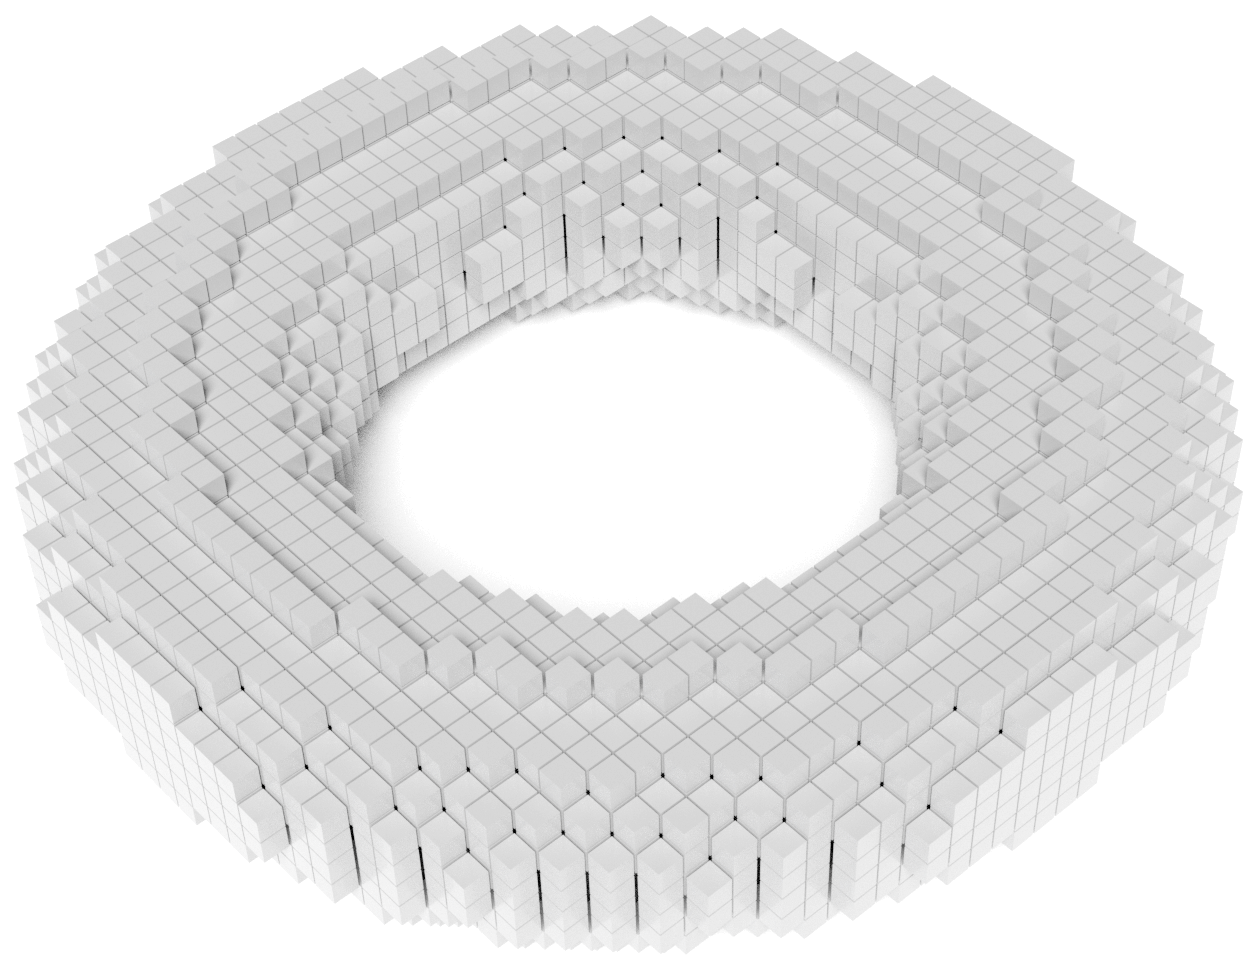
\includegraphics[width=\textwidth]{sections/result/figures/torus-voxelized-v1-40.png}
        \caption{Voxelized torus with Voxelizer v1.0.0.}
        \label{fig:result-voxelizer-v1-torus}
    \end{subfigure}
    \par\bigskip
    \begin{subfigure}[b]{0.49\textwidth}
        \centering
        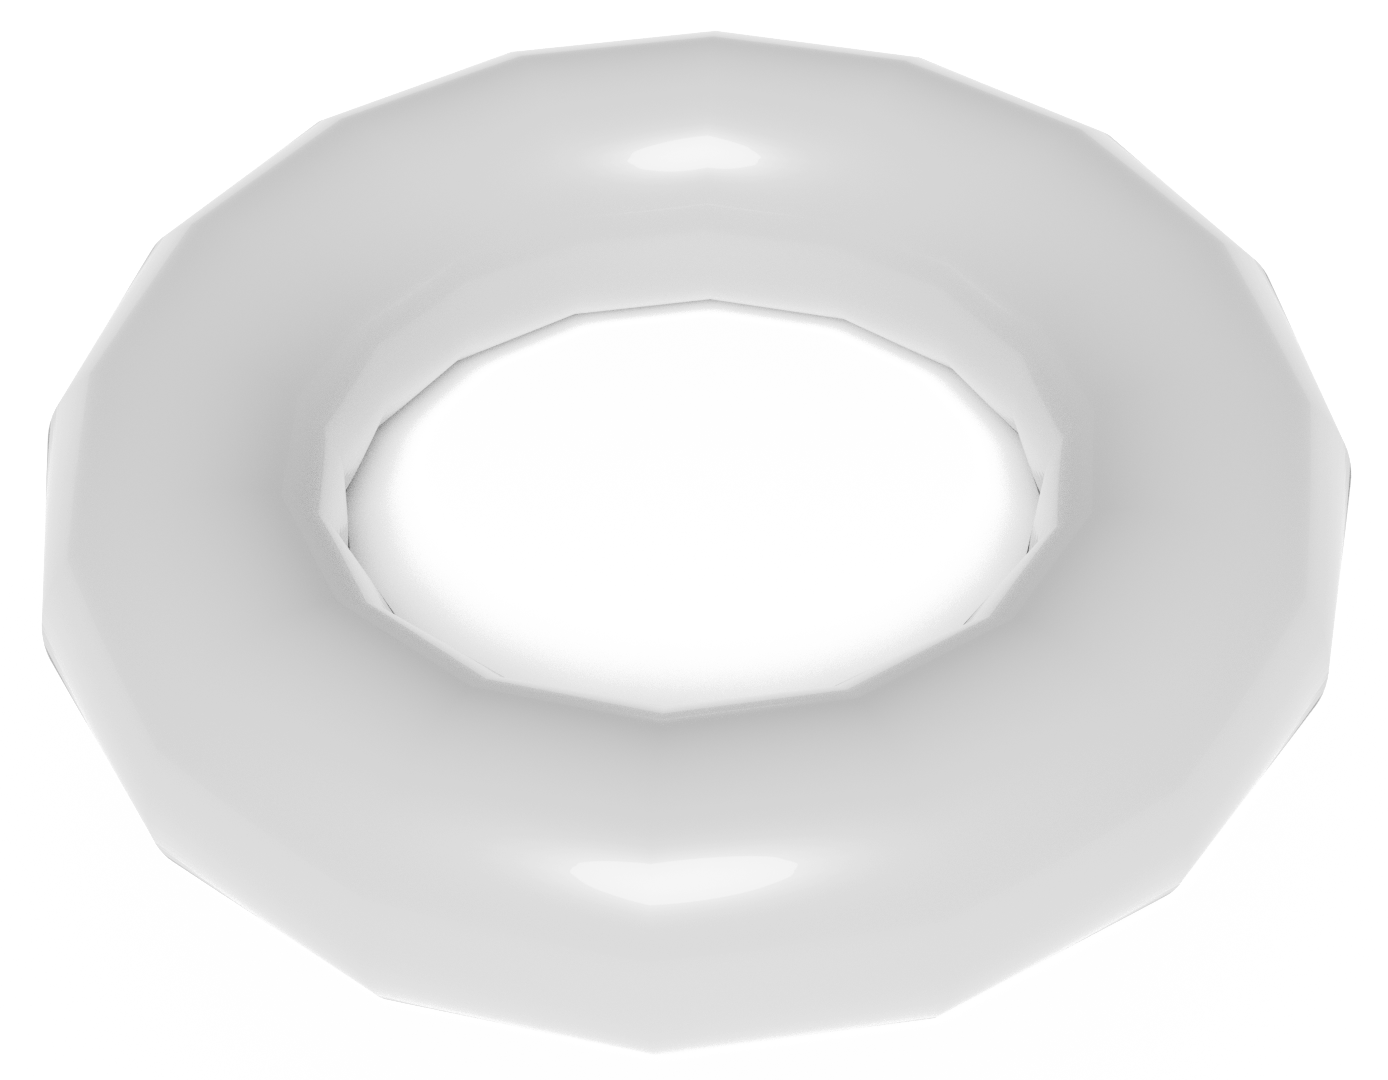
\includegraphics[width=\textwidth]{sections/theory/figures/torus.png}
        \caption{Original torus 3D model.}
        \label{fig:result-original-torus}
    \end{subfigure}
    \caption{Voxelization of a torus with Voxelizer v0.1.3 and v1.0.0. The voxelization is done with a resolution of 40.}
    \label{fig:result-voxelizer-comparison-torus}
\end{figure}
\clearpage
As mentioned in Section~\ref{sec:voxelizer-v013}, the old engine produced a lot of artifacts. The new version fixes this problem. This can be seen in Figure~\ref{fig:result-voxelizer-comparison-monkey}, which shows the voxelization of a monkey 3D model. Figure~\ref{fig:result-voxelizer-v0.1.3-monkey} shows the voxelization of a monkey with the old version, and Figure~\ref{fig:result-voxelizer-v1-monkey} shows the result with the new version. Comparing the two, it is clear that the new engine produces voxelizations where the artifacts are more or less completly removed.
\begin{figure}[hp]
    \centering
    \begin{subfigure}[b]{0.48\textwidth}
        \centering
        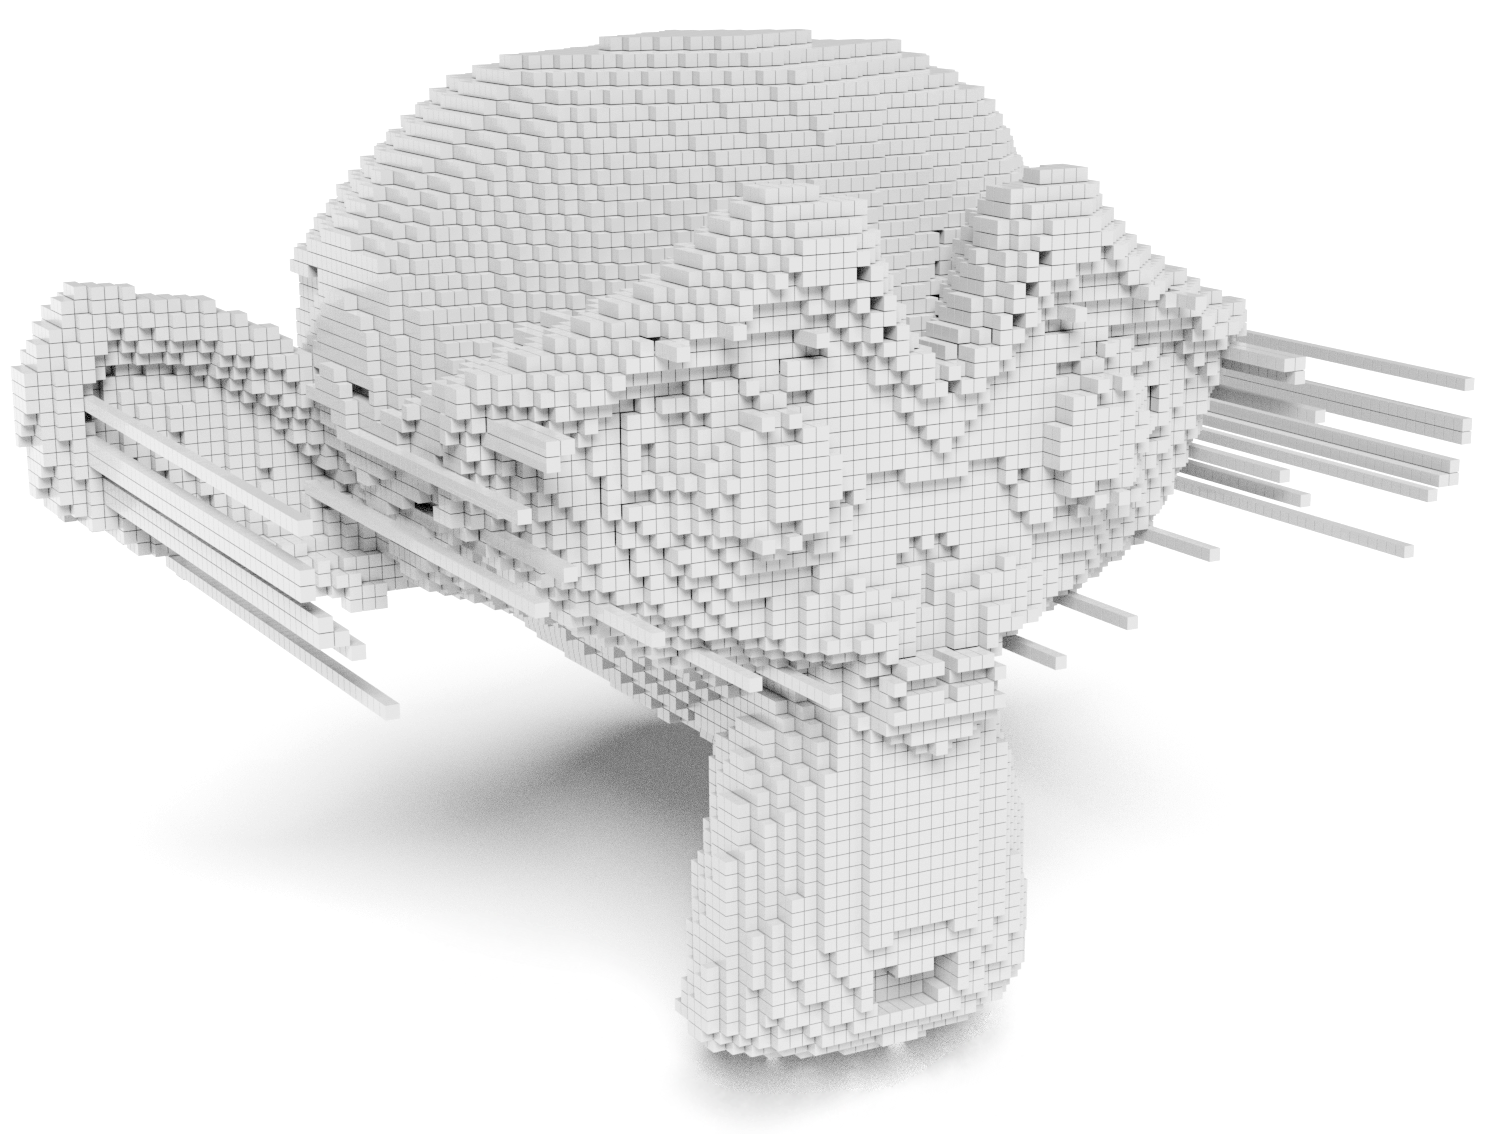
\includegraphics[width=\textwidth]{sections/theory/figures/voxelizer-v013-monkey-100.png}
        \caption{Voxelized monkey with Voxelizer v0.1.3.}
        \label{fig:result-voxelizer-v0.1.3-monkey}
    \end{subfigure}
    \hfill
    \begin{subfigure}[b]{0.50\textwidth}
        \centering
        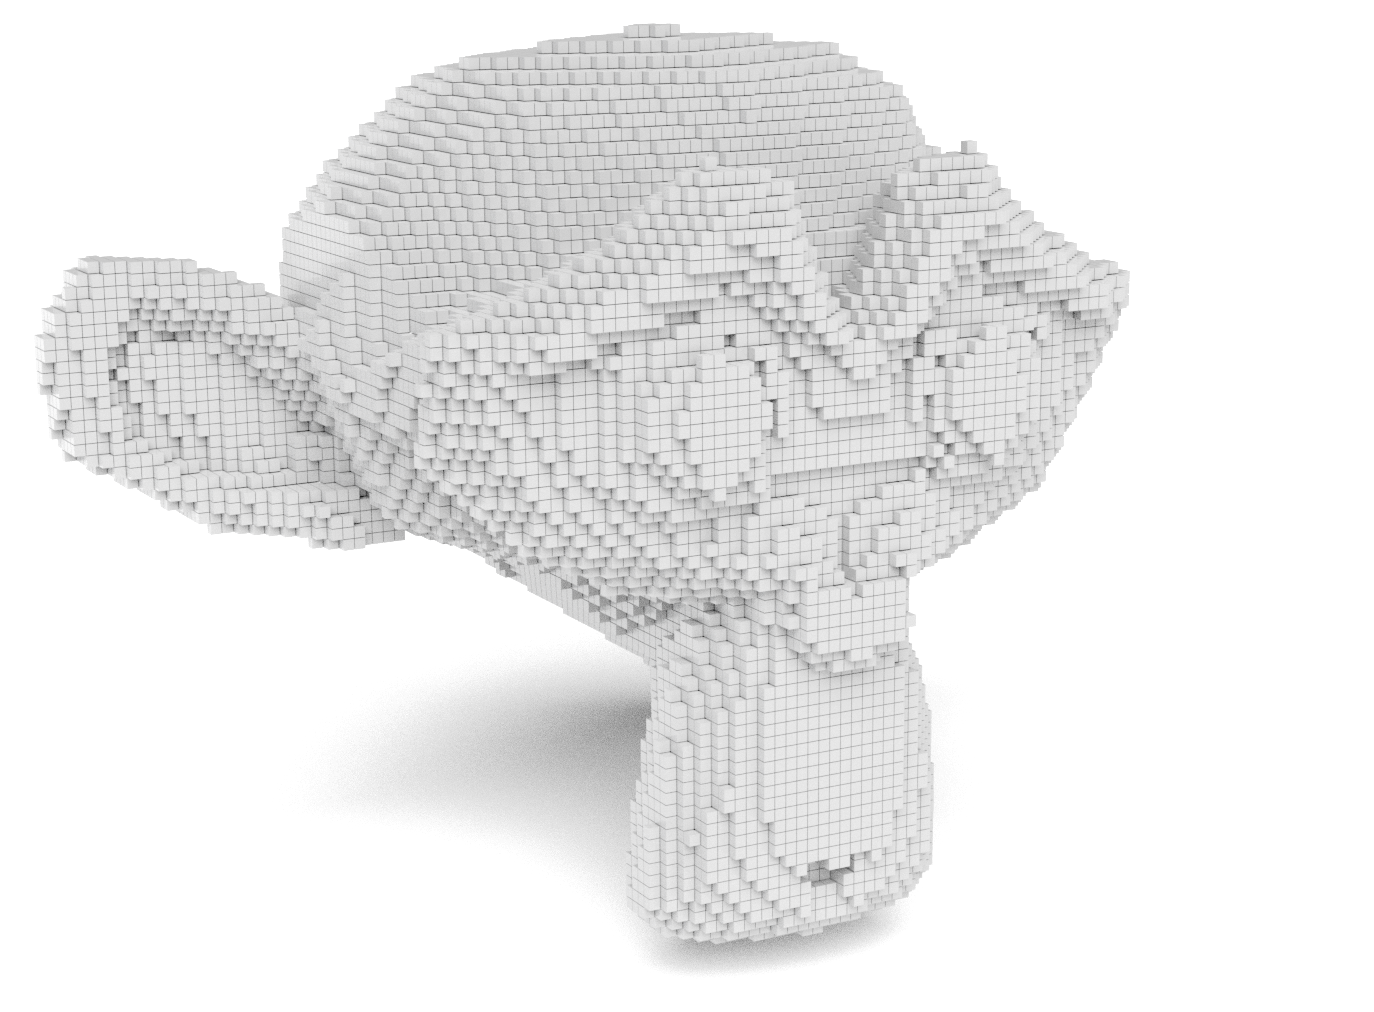
\includegraphics[width=\textwidth]{sections/result/figures/monkey-voxelized-v1-100.png}
        \caption{Voxelized monkey with Voxelizer v1.0.0.}
        \label{fig:result-voxelizer-v1-monkey}
    \end{subfigure}
    \par\bigskip
    \begin{subfigure}[b]{0.43\textwidth}
        \centering
        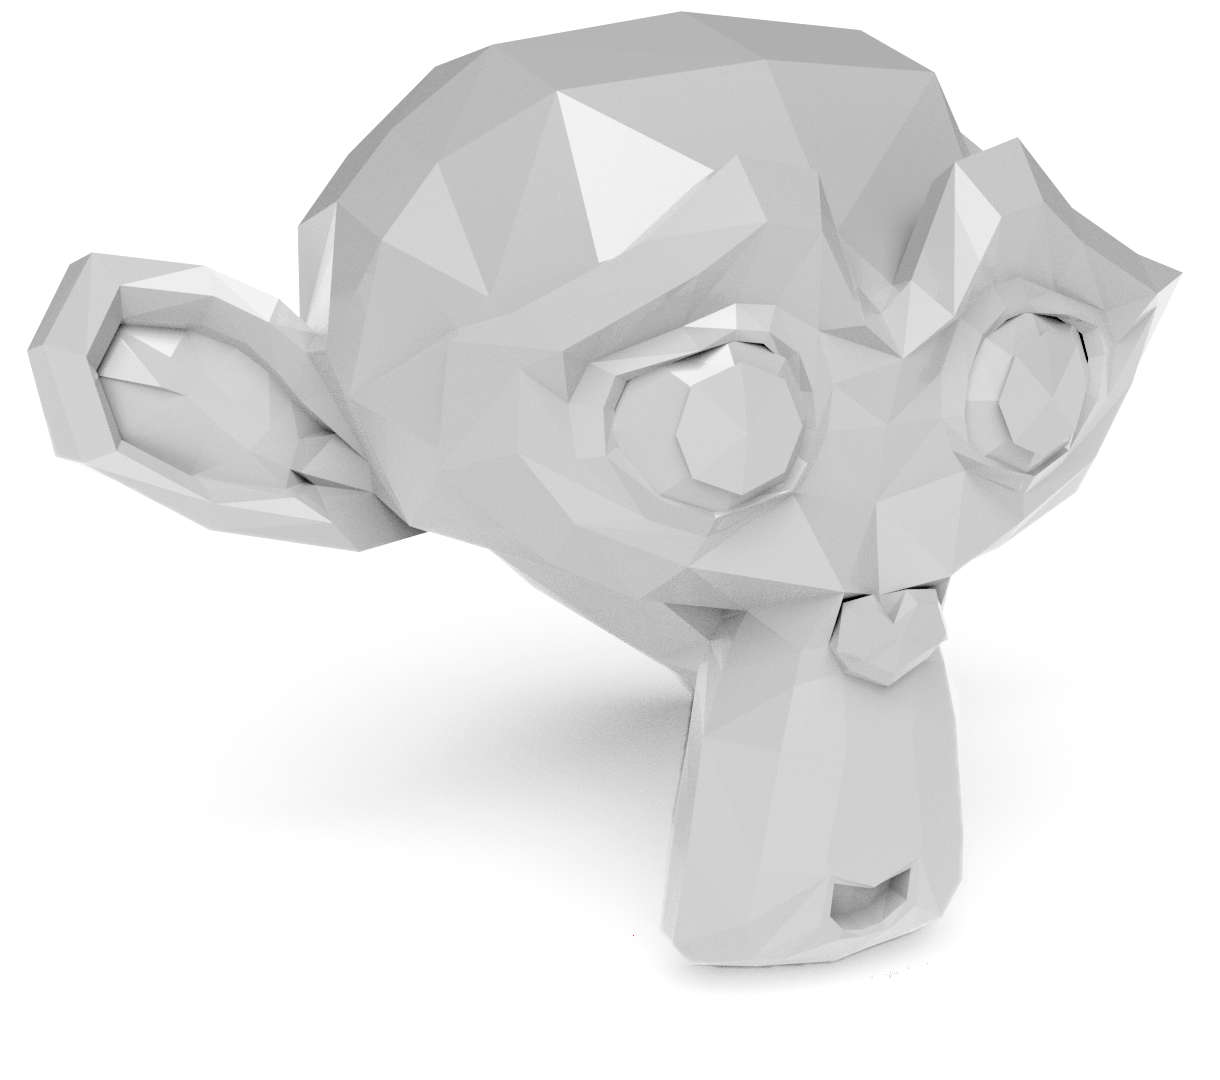
\includegraphics[width=\textwidth]{sections/theory/figures/monkey.png}
        \caption{Original monkey 3D model.}
        \label{fig:result-original-monkey}
    \end{subfigure}
    \hfill
    \caption{Voxelization of a monkey with Voxelizer v0.1.3 and v1.0.0. The voxelization is done with a resolution of 100.}
    \label{fig:result-voxelizer-comparison-monkey}
\end{figure}
\clearpage
The voxelization with the old engine often fails in filling in the gap between the sampled front and back. This produce completly unusable result. Also, since it is only sampled from the front and back, the details from the other sides of the models are not captured in the voxelization. The new version is much more robust, and captures details from all six sides of the model. This results in a much more accurate representation of the model. This improvement can clearly be seen in Figure~\ref{fig:result-voxelizer-comparison-anvil}, which shows the voxelization of an anvil 3D model. Figure~\ref{fig:result-voxelizer-v0.1.3-anvil} shows a voxelization of an anvil with the old engine. Here, the voxelization has failed in the filling process. Figure~\ref{fig:result-voxelizer-v1-anvil} shows the result with the new version. Comparing the two, it is clear that the new engine produces a lot more accureate voxelizations.
\begin{figure}[hp!]
    \centering
    \begin{subfigure}[b]{0.7\textwidth}
        \centering
        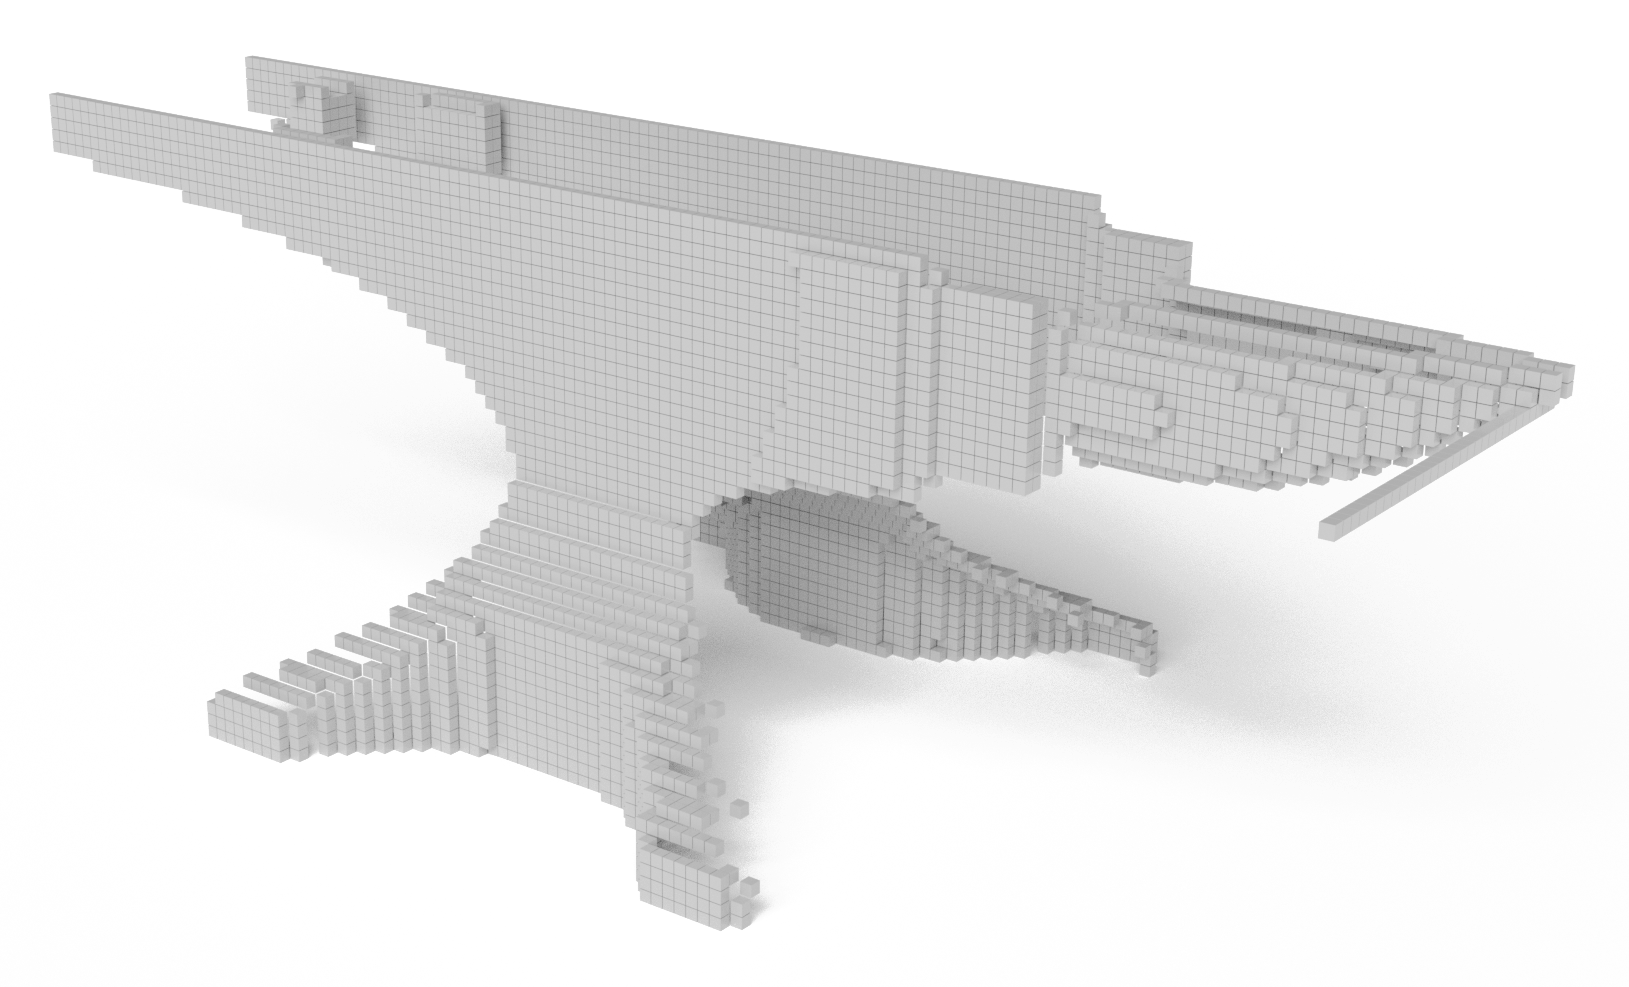
\includegraphics[width=\textwidth]{sections/theory/figures/voxelizer-v013-anvil-128.png}
        \caption{Voxelized anvil with Voxelizer v0.1.3.}
        \label{fig:result-voxelizer-v0.1.3-anvil}
    \end{subfigure}
    \\
    \begin{subfigure}[b]{0.7\textwidth}
        \centering
        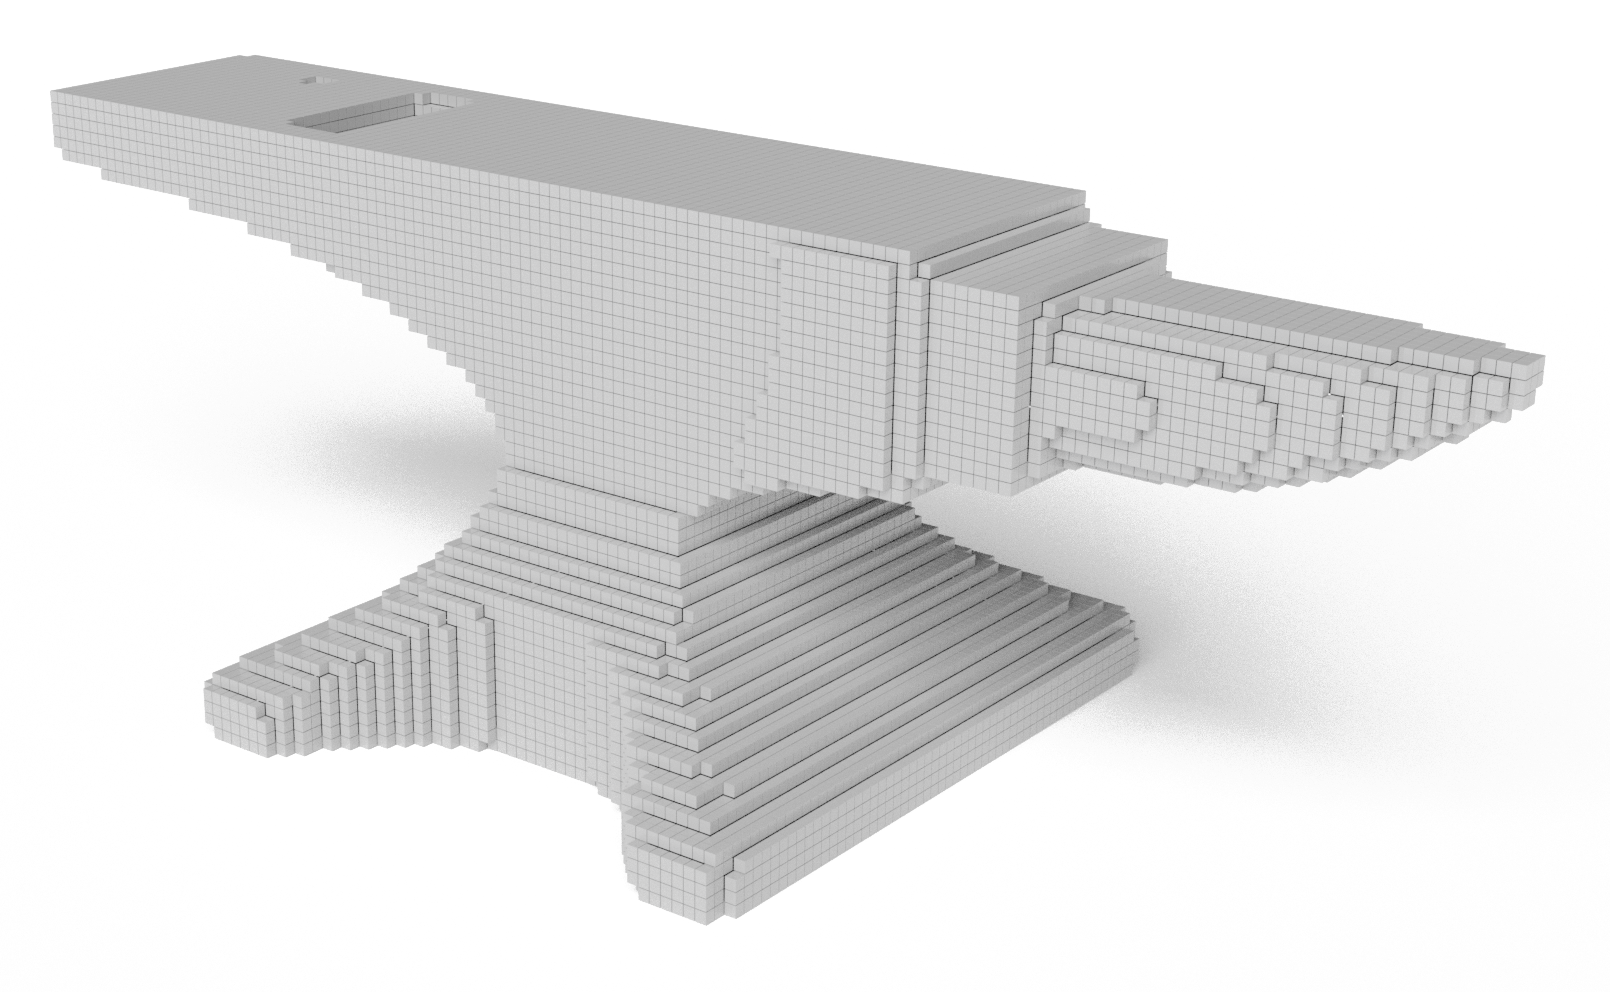
\includegraphics[width=\textwidth]{sections/result/figures/anvil-voxelized-v1-128.png}
        \caption{Voxelized anvil with Voxelizer v1.0.0.}
        \label{fig:result-voxelizer-v1-anvil}
    \end{subfigure}
    \\
    \begin{subfigure}[b]{0.7\textwidth}
        \centering
        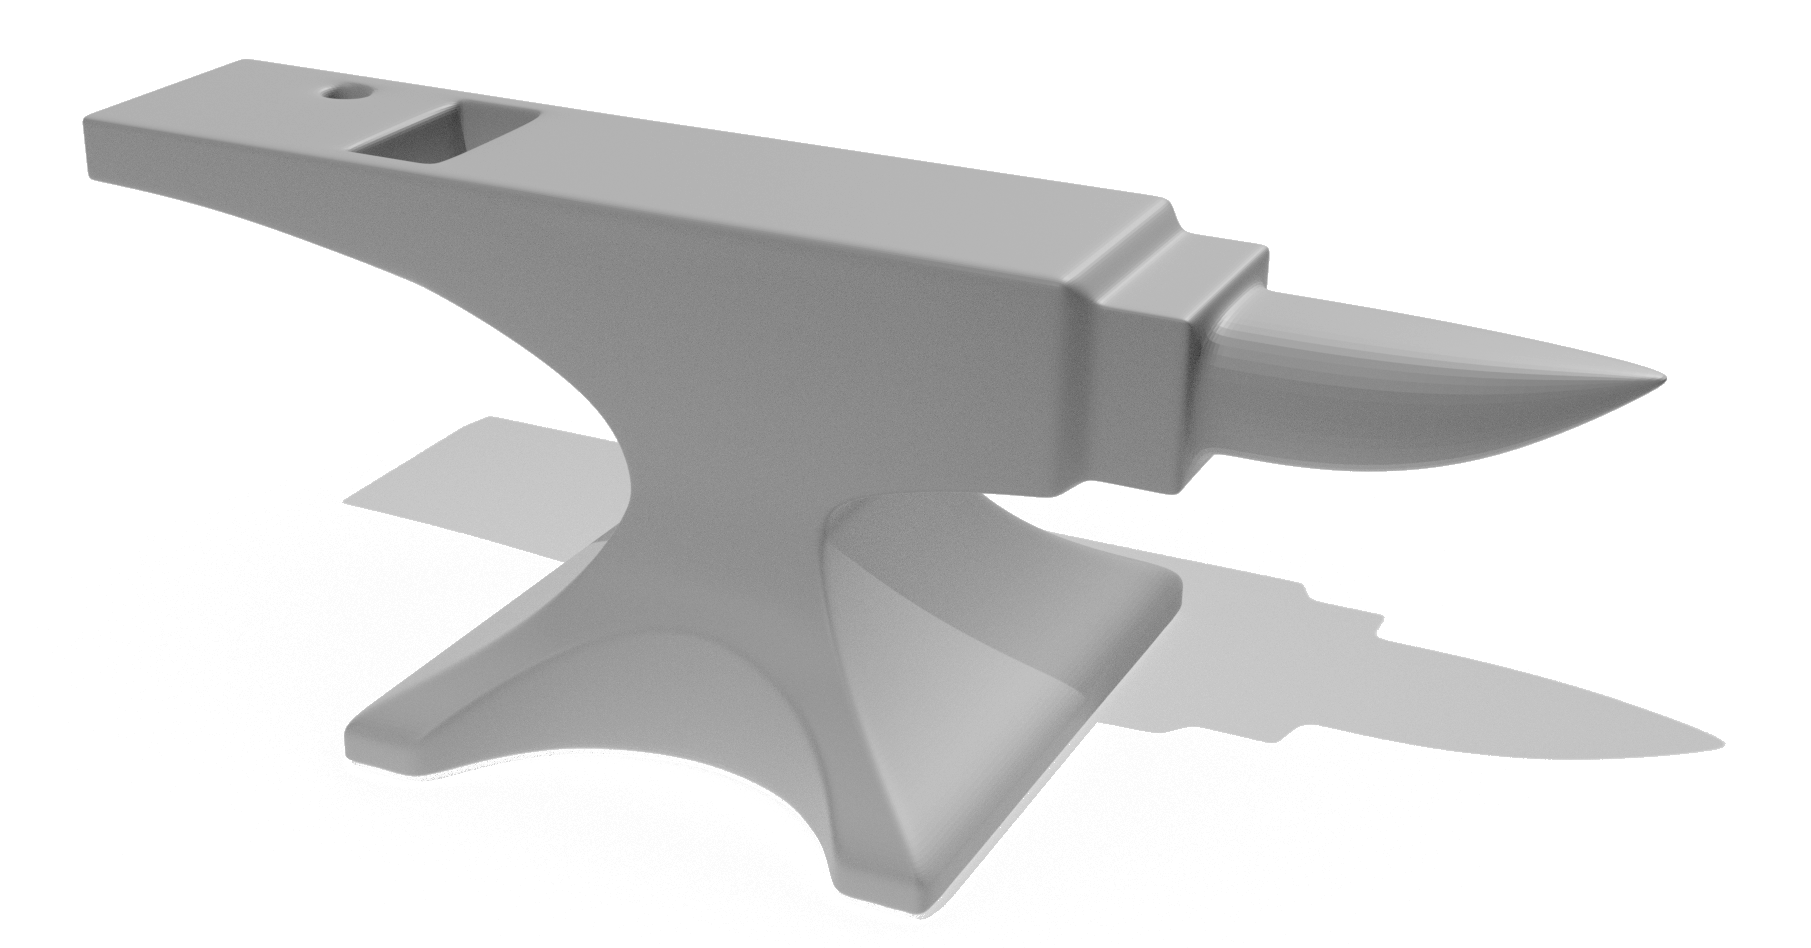
\includegraphics[width=\textwidth]{sections/theory/figures/anvil.png}
        \caption{Original anvil 3D model.}
        \label{fig:result-original-anvil}
    \end{subfigure}
    \hfill
    \caption{Voxelization of an anvil with Voxelizer v0.1.3 and v1.0.0. The voxelization is done with a resolution of $2^7$.}
    \label{fig:result-voxelizer-comparison-anvil}
\end{figure}
\clearpage
\subsection{Performance}
\label{sec:result-voxelizer-performance}
The engine's algorithm is completly overhault. The old raycasting algorithm has a time complexity of:
\[ \mathcal{O}(n^3\times m) \]
where $n$ is the resolution of the voxelization, and $m$ is the number of triangles in the 3D model. In order to produce more accurate results, the new algorithm does a lot more sampling. Despite this, the time complexity is redused. With the settings set to colorless and filled, the time complexity of the upgraded raycasting algorithm is:
\[ \mathcal{O}(n^3\times \log(m)) \]
where $n$ is the resolution of the voxelization, and $m$ is the number of triangles in the 3D model.

Following is a speed and memory comparison of the old and new vesion of the Voxelizer engine. The tests are executed in Node.js v12.16.3. The hardware used is a MacBook Pro (13-inch, 2018) with a 2.3GHz quad core processor and 16GB of 2133MHz LPDDR3 RAM, running MacOS Catalina v10.15.4.

First, the versions are tested with a low-poly mesh. Then, a high-poly mesh is used. The engine is tested at various resolutions. Note that a resolution of $2$ results in $2\times2\times2$ voxels. The old engine version is only able to do a colorless, filled voxelization. In order to make a fair comparison, the new Version's RaycastAlgorithm is set to be colorless and filled. As input, the mesh will be programatically generated by the code provided in Listing~\ref{lst:voxelizer-speed-test-mesh}. This produces a torus mesh with 3200 triangles.
\begin{lstlisting}[language=JavaScript,caption={JS code for generating low-detailed torus mesh.},label={lst:voxelizer-speed-test-mesh}]
    let geometry = new THREE.TorusBufferGeometry( 10, 3, 16, 100 );
    let material = new THREE.MeshBasicMaterial();
    let torus = new THREE.Mesh(geometry, material);
\end{lstlisting}

\clearpage
\begin{figure}[H]
    \centering
    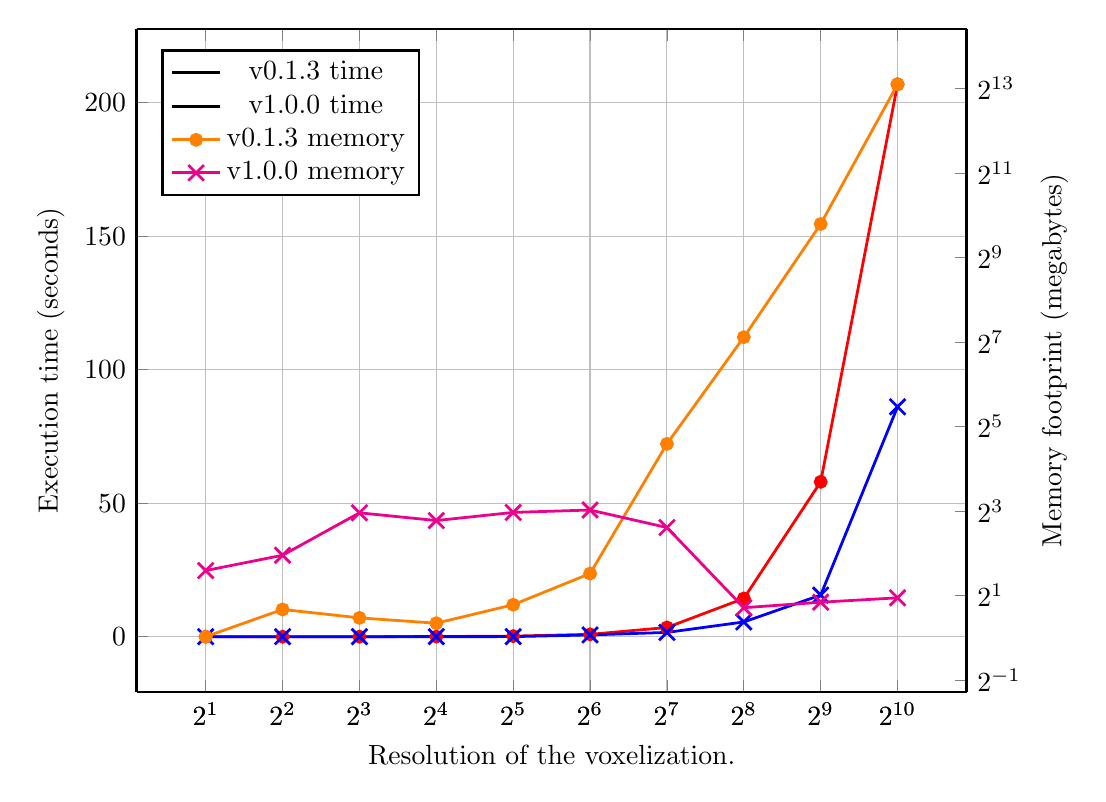
\begin{tikzpicture}
        \begin{semilogxaxis}[
            axis y line*=left,
            xlabel = Resolution of the voxelization.,
            ylabel = Execution time (seconds),
            grid=both,
            log basis x=2,
            width=\textwidth,
            height=10cm,
            ylabel near ticks,
            line width=1pt,
        ]
        \addplot[red,mark=*] coordinates {
            (2^1,  0.0254)
            (2^2,  0.0116)
            (2^3,  0.0195)
            (2^4,  0.0624)
            (2^5,  0.2288)
            (2^6,  0.8879)
            (2^7,  3.4578)
            (2^8,  14.3298)
            (2^9,  58.0136)
            (2^10, 206.8811)
        };\label{TimeOldPlot1}
        \addplot[blue,mark=x,mark size=4] coordinates {
            (2^1, 0.0154)
            (2^2, 0.0172)
            (2^3, 0.0214)
            (2^4, 0.0382)
            (2^5, 0.0403)
            (2^6, 0.6752)
            (2^7, 1.6094)
            (2^8, 5.5269)
            (2^9, 15.5968)
            (2^10, 86.0982)
        };\label{TimeNewPlot1}
        \end{semilogxaxis}
        \begin{loglogaxis}[
            axis y line*=right,
            ylabel = Memory footprint (megabytes),
            log basis x=2,
            log basis y=2,
            width=\textwidth,
            height=10cm,
            ylabel near ticks,
            line width=1pt,
            legend pos=north west
        ]
        \addlegendimage{/pgfplots/refstyle=TimeOldPlot1}\addlegendentry{v0.1.3 time}
        \addlegendimage{/pgfplots/refstyle=TimeNewPlot1}\addlegendentry{v1.0.0 time}
        \addplot[orange,mark=*] coordinates {
            (2^1,  1.0146)
            (2^2,  1.5868)
            (2^3,  1.3817)
            (2^4,  1.2659)
            (2^5,  1.7142)
            (2^6,  2.8593)
            (2^7,  24.0315)
            (2^8,  138.2336)
            (2^9,  885.5446)
            (2^10, 8764.2631)
        };\addlegendentry{v0.1.3 memory}
        \addplot[magenta,mark=x,mark size=4] coordinates {
            (2^1,  3.00344)
            (2^2,  3.8611)
            (2^3,  7.7465)
            (2^4,  6.8227)
            (2^5,  7.7983)
            (2^6,  8.1104)
            (2^7,  6.0841)
            (2^8,  1.6326)
            (2^9,  1.7861)
            (2^10, 1.9199)
        };\addlegendentry{v1.0.0 memory}
        \end{loglogaxis}
    \end{tikzpicture}
    \caption{Plot over execution time and memory footprint for voxelization of a low-detailed mesh with the old and new Voxelizer engine.}
    \label{fig:plot-execution-time-low-poly}
\end{figure}
\begin{table}[H]
    \newcolumntype{Y}{>{\centering\arraybackslash}X}
    \begin{minipage}[t]{.45\linewidth}
        \centering
        \caption{Execution times and memory footprints for voxelization of low-detailed mesh with Voxelizer v0.1.3.}
        \label{tab:performance-voxelizer-v0.1.3-low-poly}
        \medskip
        \begin{tabularx}{\textwidth}{*{3}{|Y}|}
            \hline
            \textbf{Resolution}& \textbf{Time (sec)} & \textbf{Memory (MB)}\\
            \hline
            2\textsuperscript{1} & 0.0254 & 1.0146 \\
            2\textsuperscript{2} & 0.0116 & 1.5868 \\
            2\textsuperscript{3} & 0.0195 & 1.3817 \\
            2\textsuperscript{4} & 0.0624 & 1.2659 \\
            2\textsuperscript{5} & 0.2288 & 1.7142 \\
            2\textsuperscript{6} & 0.8879 & 2.8593 \\
            2\textsuperscript{7} & 3.4578 & 24.0315 \\
            2\textsuperscript{8} & 14.3298 & 138.2336 \\
            2\textsuperscript{9} & 58.0136 & 885.5446 \\
            2\textsuperscript{10} & 260.8811 & 8764.2631 \\
            \hline
        \end{tabularx}
    \end{minipage}\hfill
    \begin{minipage}[t]{.45\linewidth}
        \centering
        \caption{Execution times and memory footprints for voxelization of low-detailed mesh with Voxelizer v1.0.0.}
        \label{tab:performance-voxelizer-v1.0.0-low-poly}
        \medskip
        \begin{tabularx}{\textwidth}{*{3}{|Y}|}
            \hline
            \textbf{Resolution} & \textbf{Time (sec)} & \textbf{Memory (MB)}\\
            \hline
            2\textsuperscript{1} & 0.0154 & 3.00344\\
            2\textsuperscript{2} & 0.0172 & 3.8611\\
            2\textsuperscript{3} & 0.0214 & 7.7465\\
            2\textsuperscript{4} & 0.0382 & 6.8227\\
            2\textsuperscript{5} & 0.0403 & 7.7983\\
            2\textsuperscript{6} & 0.6752 & 8.1104\\
            2\textsuperscript{7} & 1.6094 & 6.0841\\
            2\textsuperscript{8} & 5.5269 & 1.6326\\
            2\textsuperscript{9} & 15.5968 & 1.7861\\
            2\textsuperscript{10} & 86.0982 & 1.9199\\
            \hline
        \end{tabularx}
    \end{minipage}
\end{table}

Figure~\ref{fig:plot-execution-time-low-poly} shows a graph over the execution time and the memory footprint for a voxelization of a low-detailed mesh with the Voxelizer engine v0.1.3 and v1.0.0. The raw data is available in Table~\ref{tab:performance-voxelizer-v0.1.3-low-poly} and Table~\ref{tab:performance-voxelizer-v1.0.0-low-poly}.

The new engine has a relatively low memory footprint. At resolutions from $2^1$ to $2^7$, the memory consumption stays around 7MB. Then, at a resolution of $2^8$, the memory drops to around 2MB. This is most likely due to the JavaScript Garbage Collector (GC) kicking in. At larger resolutions, the memory seems to stay relatively stabile around 2MB. The old engine starts with a very low memory footprint. It stays low, between 1MB and 2MB, from a resolution of $2^1$ to $2^6$. Then, the memory footprint starts to increase rapidly. A total of 24MB are used for a resolution of $2^7$. At $2^{10}$ the footprint has risen to 8.7GB. This is most likely due to the fact that the old engine used normal JavaScript arrays that dynamically expands. A lot of obsolete data objects will accumulate, and the GC seems to not be able to handle this well.

Regarding execution time, this is also greatly improved in the new engine version. This is especially noticeable at large resolutions. At a resolution of $2^{10}$, the old engine use 260 seconds to voxelize the 3D model. The new version only use 86 seconds, a reduction of about $60\%$.

An new mesh is generated with the code in Listing~\ref{lst:voxelizer-speed-test-mesh-high}. This produces a highly detailed torus mesh with 1,000,000 triangles. The results are presented in the figures below.

\begin{lstlisting}[language=JavaScript,caption={JS code for generating high-detailed torus mesh.},label={lst:voxelizer-speed-test-mesh-high}]
let geometry = new THREE.TorusBufferGeometry( 10, 3, 1000, 500 );
let material = new THREE.MeshBasicMaterial();
let torus = new THREE.Mesh(geometry, material);
\end{lstlisting}
\clearpage
\begin{figure}[H]
    \centering
    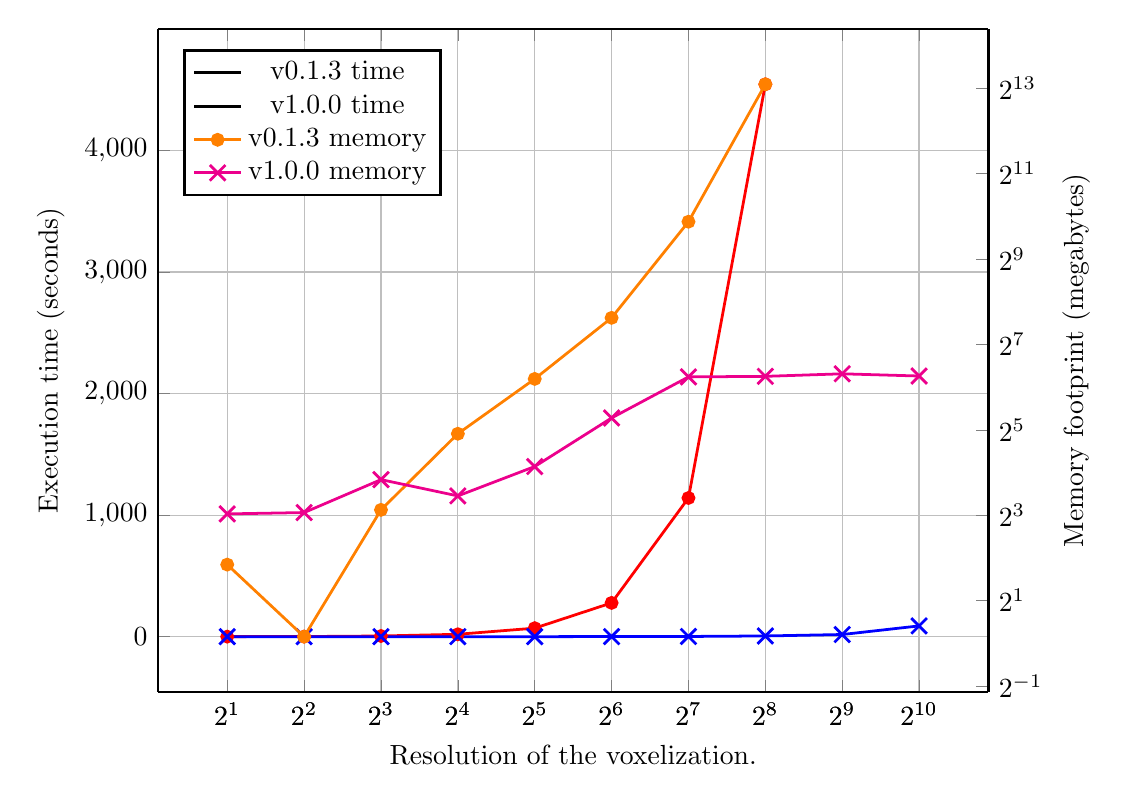
\begin{tikzpicture}
        \begin{semilogxaxis}[
            axis y line*=left,
            xlabel = Resolution of the voxelization.,
            ylabel = Execution time (seconds),
            grid=both,
            log basis x=2,
            width=\textwidth,
            height=10cm,
            ylabel near ticks,
            line width=1pt,
        ]
        \addplot[red,mark=*] coordinates {
            (2^1,  0.5388)
            (2^2,  1.2370)
            (2^3,  5.8674)
            (2^4,  19.8983)
            (2^5,  70.2835)
            (2^6,  278.1215)
            (2^7,  1141.1212)
            (2^8,  4543.6064)
        };\label{TimeOldPlot2}
        \addplot[blue,mark=x,mark size=4] coordinates {
            (2^1, 0.17265)
            (2^2, 0.1612)
            (2^3, 0.2277)
            (2^4, 0.2755)
            (2^5, 0.3402)
            (2^6, 1.0793)
            (2^7, 1.9604)
            (2^8, 6.0971)
            (2^9, 17.9376)
            (2^10, 88.8092)
        };\label{TimeNewPlot2}
        \end{semilogxaxis}
        \begin{loglogaxis}[
            axis y line*=right,
            ylabel = Memory footprint (megabytes),
            log basis x=2,
            log basis y=2,
            width=\textwidth,
            height=10cm,
            ylabel near ticks,
            line width=1pt,
            legend pos=north west
        ]
        \addlegendimage{/pgfplots/refstyle=TimeOldPlot2}\addlegendentry{v0.1.3 time}
        \addlegendimage{/pgfplots/refstyle=TimeNewPlot2}\addlegendentry{v1.0.0 time}
        \addplot[orange,mark=*] coordinates {
            (2^1,  3.5880)
            (2^2,  1.1134)
            (2^3,  8.7263)
            (2^4,  30.0106)
            (2^5,  73.1078)
            (2^6,  197.0107 )
            (2^7,  937.7180 )
            (2^8,  8726.9914)
        };\addlegendentry{v0.1.3 memory}
        \addplot[magenta,mark=x,mark size=4] coordinates {
            (2^1,  8.1706)
            (2^2,  8.3496)
            (2^3,  14.2518)
            (2^4,  10.9389)
            (2^5,  17.6270)
            (2^6,  38.7798)
            (2^7,  75.5248)
            (2^8,  76.1971)
            (2^9,  79.4146)
            (2^10, 76.6116)
        };\addlegendentry{v1.0.0 memory}
        \end{loglogaxis}
    \end{tikzpicture}
    \caption{Plot over execution time and memory footprint for voxelization of a high-detailed mesh with the old and new Voxelizer engine.}
    \label{fig:plot-execution-time-high-poly}
\end{figure}
\begin{table}[ht]
    \newcolumntype{Y}{>{\centering\arraybackslash}X}
    \def\arraystretch{1.5}
    \begin{minipage}[t]{.45\linewidth}
        \centering
        \caption{Execution times and memory footprints for voxelization of high-detailed mesh with Voxelizer v0.1.3.}
        \label{tab:performance-voxelizer-v0.1.3-high-poly}
        \medskip
        \begin{tabularx}{\textwidth}{*{3}{|Y}|}
            \hline
            \textbf{Resolution}& \textbf{Time (sec)} & \textbf{Memory (MB)}\\
            \hline
            2\textsuperscript{1} & 0.5388 & 3.5880\\
            2\textsuperscript{2} & 1.2370 & 1.1134\\
            2\textsuperscript{3} & 5.8674 & 8.7263\\
            2\textsuperscript{4} & 19.8983 & 30.0106\\
            2\textsuperscript{5} & 70.2835 & 73.1078\\
            2\textsuperscript{6} & 278.1215 & 197.0107 \\
            2\textsuperscript{7} & 1141.1212 & 937.7180 \\
            2\textsuperscript{8} & 4543.6064 & 8726.9914\\
            \hline
        \end{tabularx}
    \end{minipage}\hfill
    \begin{minipage}[t]{.45\linewidth}
        \centering
        \caption{Execution times and memory footprints for voxelization of high-detailed mesh with Voxelizer v1.0.0.}
        \label{tab:performance-voxelizer-v1.0.0-high-poly}
        \medskip
        \begin{tabularx}{\textwidth}{*{3}{|Y}|}
            \hline
            \textbf{Resolution} & \textbf{Time (sec)} & \textbf{Memory (MB)}\\
            \hline
            2\textsuperscript{1} & 0.17265 & 8.1706\\
            2\textsuperscript{2} & 0.1612 & 8.3496\\
            2\textsuperscript{3} & 0.2277 & 14.2518\\
            2\textsuperscript{4} & 0.2755 & 10.9389\\
            2\textsuperscript{5} & 0.3402 & 17.6270\\
            2\textsuperscript{6} & 1.0793 & 38.7798\\
            2\textsuperscript{7} & 1.9604 & 75.5248\\
            2\textsuperscript{8} & 6.0971 & 76.1971\\
            2\textsuperscript{9} & 17.9376 & 79.4146\\
            2\textsuperscript{10} & 88.8092 & 76.6116\\
            \hline
        \end{tabularx}
    \end{minipage}
\end{table}

Figure~\ref{fig:plot-execution-time-high-poly} shows a graph over the execution time and the memory footprint for a voxelization of a high-detailed mesh with the Voxelizer engine v0.1.3 and v1.0.0. The raw data is available in Table~\ref{tab:performance-voxelizer-v0.1.3-high-poly} and Table~\ref{tab:performance-voxelizer-v1.0.0-high-poly}.

The results shows similar characteristics as the ones with the low detailed mesh. However, very noticeable is the large difference in execution time. At a resolution of $2^{7}$, the old version is able to voxelize the mesh with 1,000,000 triangles in 4543 seconds, about 75 minutes. The new version is able to do the same in only about 6.1 second. The new version is also tested at a resolution of $2^{10}$. This takes only 88.8 seconds. This massive performance improvement is mainly due to the raycasting optimization discussed in Section~\ref{sec:three.js-optimization}.

The memory consumption of the old version is more or less the same as with a low detailed mesh. The new version does consume more memory than in the previous test. This is because the BVH tree generated for the raycasting performance improvement does need a bit of memory. The memory footprint of the new version seems to gradually scale up from 8MB at a resolution of $2^1$, to 76MB at resolution $2^7$. From here on, the memory footprint stay more or less constant. This is because the BVH implementation gradually builds up the BVH tree, as described in Section~\ref{sec:three.js-optimization}.

\subsection{Exporting}
Several new exporting options are added to the upgraded Voxelizer engine. This includes XML, BINVOX and ndarray. The old multidimensional JavaScript array exporting option is also available, ensuring some backwards compatibility. The exporters system is made extensible, making it easy to add new exporting options in the future.

\subsection{Code quality}
This section describes how the code quality is improved. The old codebase had several problems. Firstly, all the code was contained in one large file. This made it hard to navigate and the code was messy. The new version makes use of ES Modules, making it possible to organize the code in different files. Secondly, the engine previously hardcoded the one algorithm used. The new version includes an easily extensible algorithm system. This is ensured through the use of inheritance and factory patterns, as discussed in Section~\ref{sec:method-algorithm-system}. Thirdly, the code did barely include tests for the system. The new version now includes unit tests for almost the whole engine. Lastly, the code had no code documentation. This is resolved by writing JSDoc for all classes and functions. This \href{https://andstor.github.io/voxelizer/}{documentation} is also made easily accessible at GitHub Pages with the help of the new JSDoc Action, presented in Section~\ref{sec:result-jsdoc-action}. A screenshot of the public documentation page is shown in Figure~\ref{fig:result-voxelizer-documentation}.
\begin{figure}[htp]
    \centering
    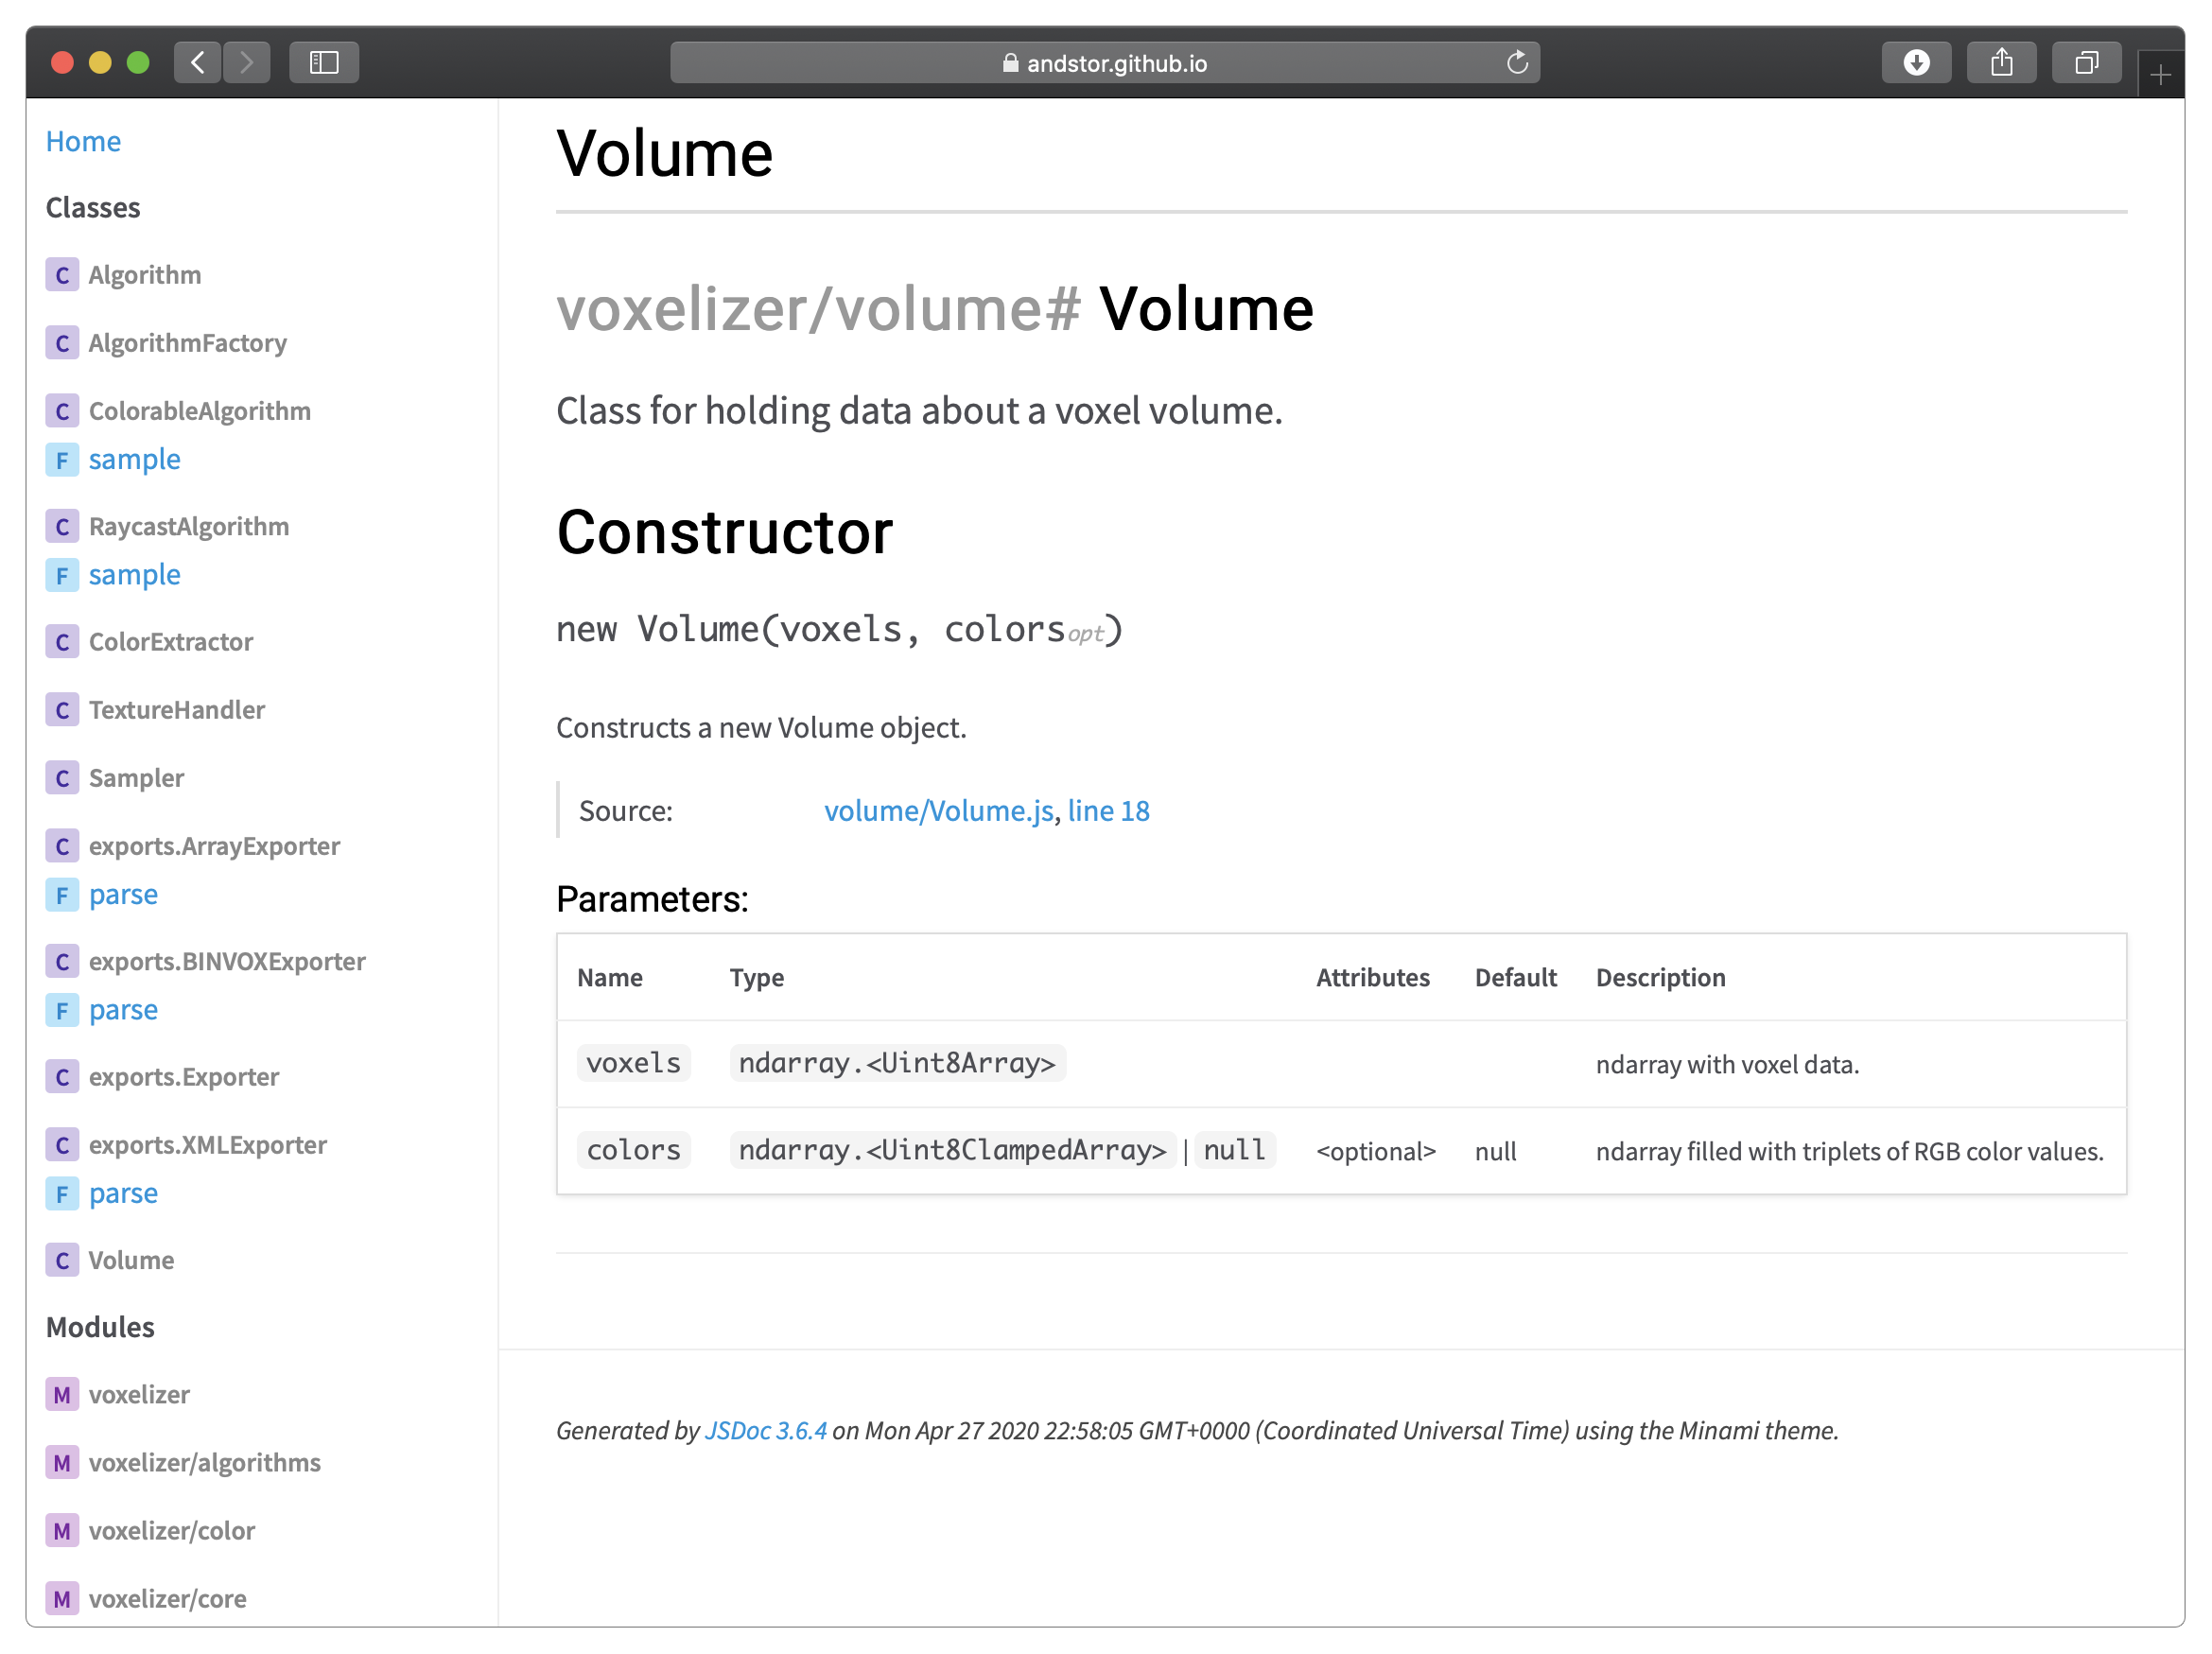
\includegraphics[width=0.9\textwidth]{sections/result/figures/voxelizer-documentation.png}
    \caption{Public documentation for the Voxelizer engine.}
    \label{fig:result-voxelizer-documentation}
\end{figure}

\subsection{Example}
An example of the engine is deployed to GitHub Pages. Visit \url{https://andstor.github.io/voxelizer/examples/} to see the example. Figure~\ref{fig:voxelizer-example} shows a screenshot of the site. The example includes a GUI with controls for controlling, among other things, the resolution, shell or solid voxelization, the LOD, and clipping planes for visually inspecting the results.
\begin{figure}[ht]
    \centering
    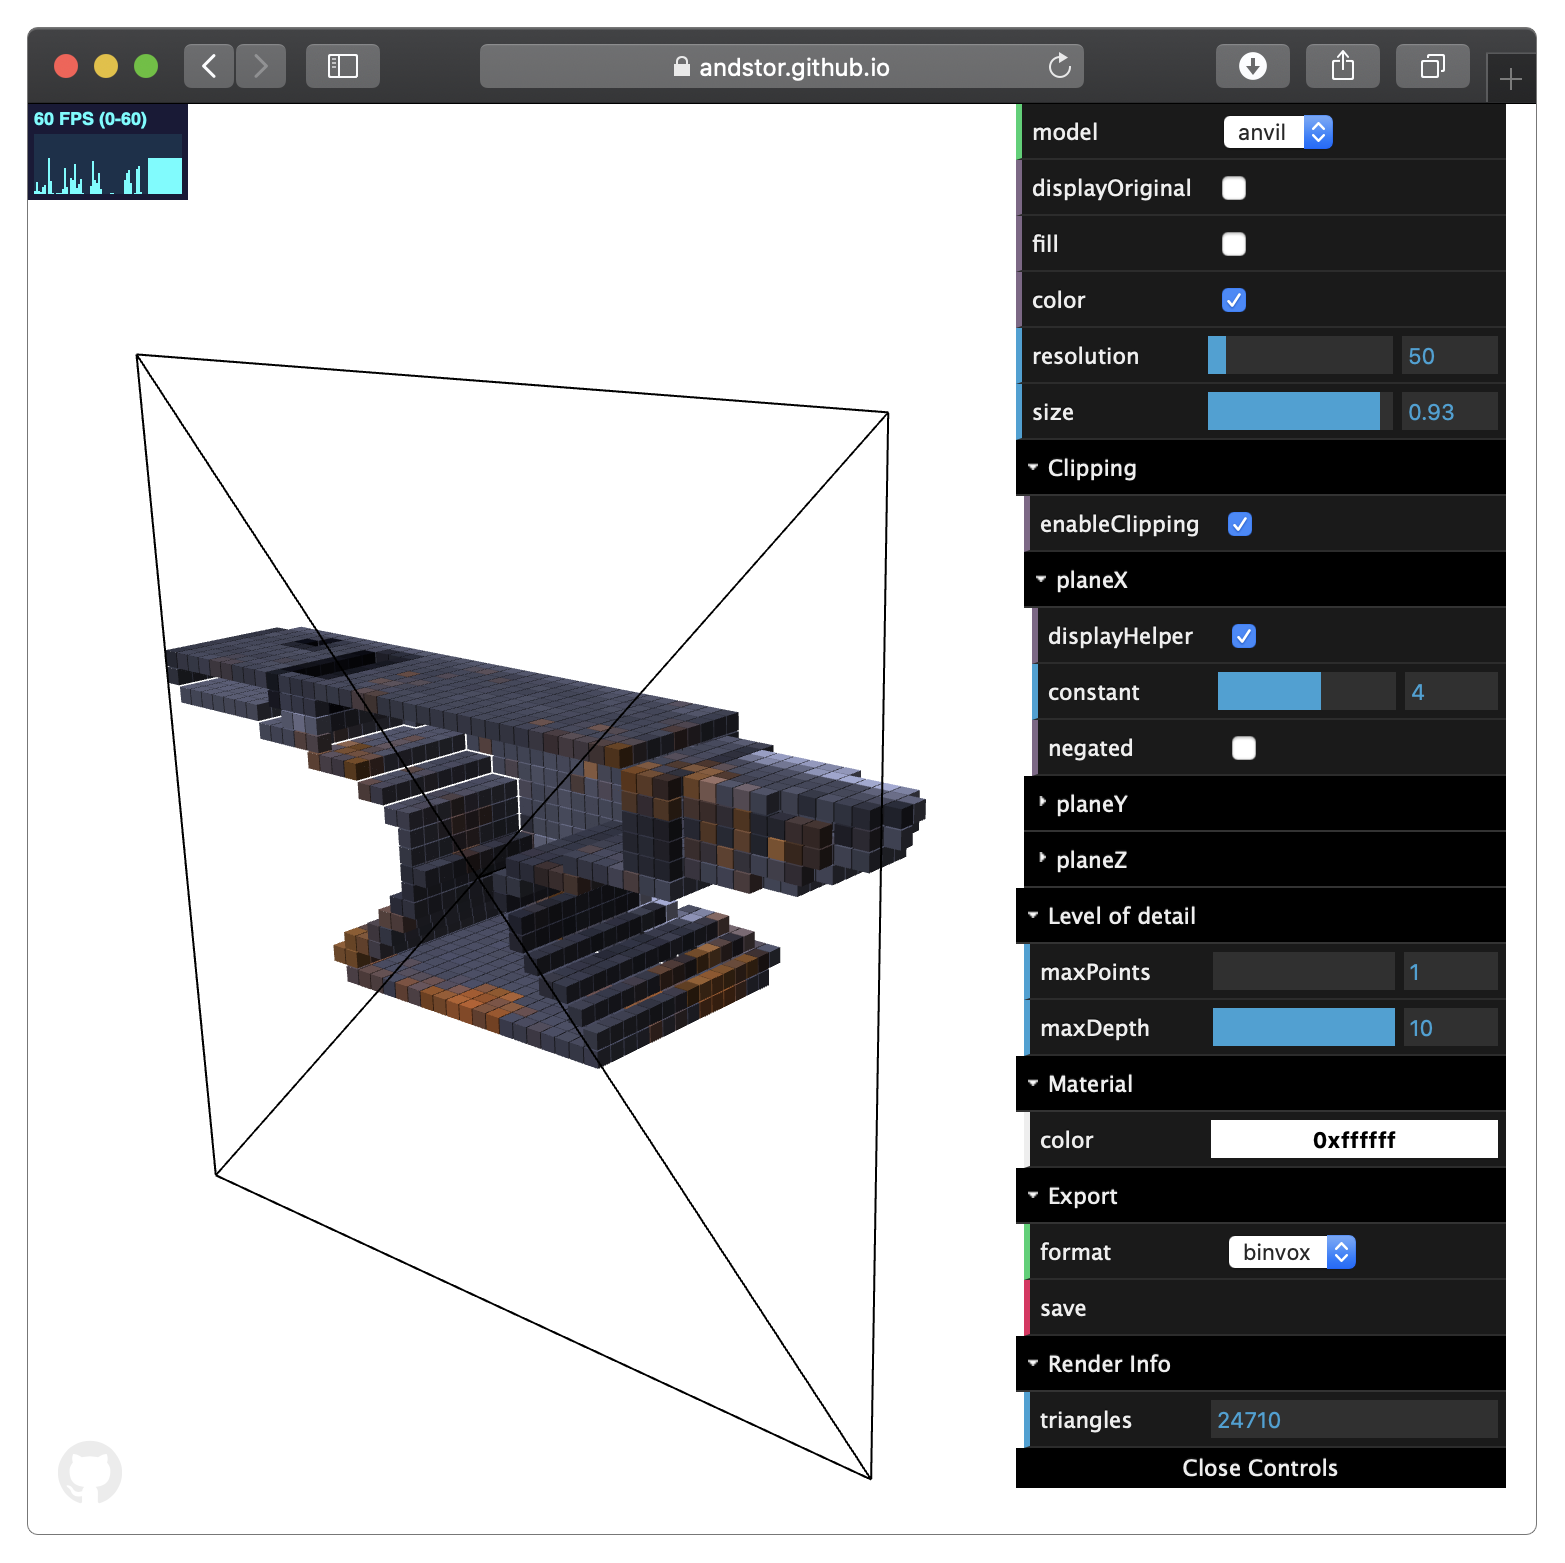
\includegraphics[width=0.9\textwidth]{sections/result/figures/voxelizer-example.png}
    \caption{Screenshot of the Voxelizer engine example page at GitHub Pages.}
    \label{fig:voxelizer-example}
\end{figure}

\clearpage
\subsection{Usage example}
This section provides an example of how to use the Voxelizer engine v1.0.0. This example assumes that the project is bundled with a tool such as Webpack or Browserify, enabling the use of the ES Modules import syntax. Also, the node package manager (npm) is assumed to be installed.

First, the engine and its peer dependency three.js needs to be installed. This is easily done with npm. To install the Voxelizer engine and the peer dependency three.js, run the following commands:
\begin{verbatim}
    $ npm install voxelizer
    $ npm install three
\end{verbatim}
Then, Listing~\ref{voxelizer-engine-example} provides the example code now to be described in steps: 
\begin{enumerate}
    \item First, the Voxelizer engine v1.0.0, and its peer dependency three.js needs to be imported. This is done in lines 2 and 3.
    \item Line 4 imports the GLTFLoader. This makes it possible to load a GLTF file.
    \item Then something to voxelized is needed. This could be any three.js mesh with BufferGeometry. By using the imported GLTFLoader, a GLTF file can be loaded. The GLTFLoader is instantiated on line 7.
    \item To actually load the model, the asynchronous "load" function is used at line 8. This function needs a path to the file to load.
    \item To set up the Voxelizer sampling class, some options are needed. These are defined on lines 12-15, making the engine produce a colored shell voxelization.
    \item The sampler is then instantiated at line 16.
    \item Line 19 and 20 actually samples the model with a resolution of 10.
    \item In order to inspect the results, the returned volume data is fed to a XMLExporter at lines 23-26. This converts the volume data to a XML resource.
    \item Line 25 prints the XML output to the console.
\end{enumerate}
The result of the example code is a $10^3$ voxel result of the loaded 3D model.

\lstinputlisting[language=JavaScript,style=numbers,label={voxelizer-engine-example}, caption={Voxelizer engine v1.0.0 example usage.}]{sections/result/code/voxelizer.js}
\clearpage

\section{BINVOX}
BINVOX is a package for parsing and building BINVOX files. It is published to the npm registry under the name "\href{https://www.npmjs.com/package/binvox}{binvox}", and the source code is available at GitHub under "\href{https://github.com/andstor/binvox}{andstor/binvox}".

The package handles BINVOX files according to the BINVOX file format specification~\cite{binvox-file-format}. The package is able to parse a BINVOX resource, turning it into JSON. Further, it can do this in reverse. Hence, properly formatted JSON data can be turned into a BINVOX file resource. The package provides both an ES Module build and a UMD build. It can therefore be used with both Node.js and in the browser.

\section{Voxelizer Desktop}
The Voxelizer Desktop application allows for easy use of the Voxelizer engine. It is a standalone cross platform desktop application. Ready-made installation files for macOS, Windows and Linux can be found at \url{https://github.com/andstor/voxelizer-desktop/releases/latest} on GitHub. The source code is also available at GitHub under "\href{https://github.com/andstor/voxelizer-desktop}{andstor/voxelizer-desktop}".

\subsection{Features}
The Voxelizer Desktop application includes several features.
\begin{itemize}
    \item \textbf{Importing} - The application supports several 3D model file formats. This includes GLB, GLTF, OBJ and STL. Some data formats need additional resources like texture images or binaries in order to work. This is also supported.
    \item \textbf{Voxelization} - The Voxelizer engine provides the application with voxelization capabilities. Several voxelization options are available, including: resolution, coloring and filling.
    \item \textbf{Visualization} - It is possible to view and inspect both the loaded 3D model and voxelized result through an interactive window.
    \item \textbf{Exporting} - Voxelizer Desktop enables the user to export to a XML file or a BINVOX file, and save this to the file system.
    \item \textbf{Auto updating} - When a new version of the application is released on GitHub, the application will automatically download and install the new version.
\end{itemize}

\subsection{GUI}
The user is first presented with an elegant and easy drag and drop user interface. Here, the user can just drop the 3D model files. Figure~\ref{fig:voxelizer-desktop-gui-dnd} shows a screenshot of the start screen, where a file is dropped onto the window.
\begin{figure}[htp]
    \centering
    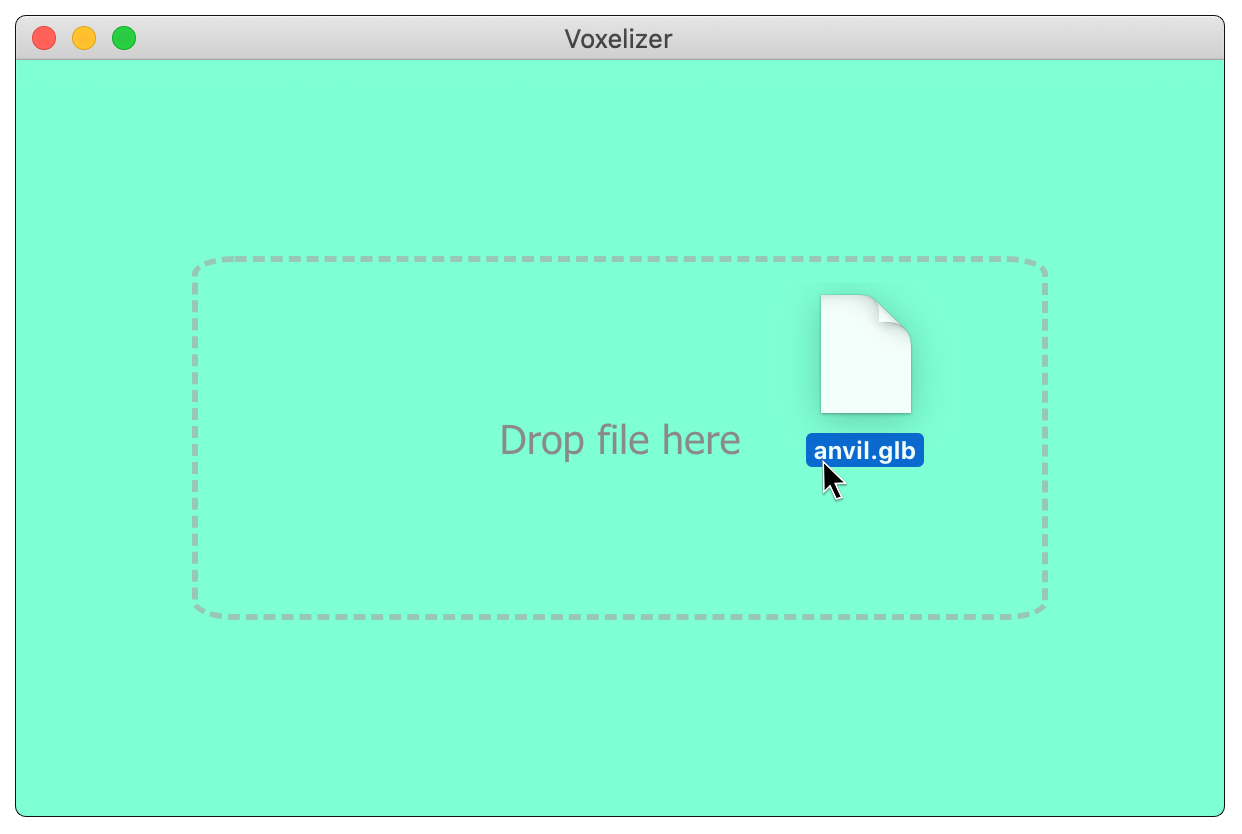
\includegraphics[width=0.9\textwidth]{sections/result/figures/voxelizer-desktop-gui-dnd.png}
    \caption{Voxelizer Desktop drag and drop start screen.}
    \label{fig:voxelizer-desktop-gui-dnd}
\end{figure}

When a user drops one or more files, the application starts to load them up. If no supported filetype is found, a modal warning shows up like the one seen in Figure~\ref{fig:voxelizer-desktop-gui-dnd-file-warning}. Otherwise, a spinning loading wheel is presented, as shown in Figure~\ref{fig:voxelizer-desktop-gui-loading}, to indicate that the 3D model is loading.

\begin{figure}[htp]
    \centering
    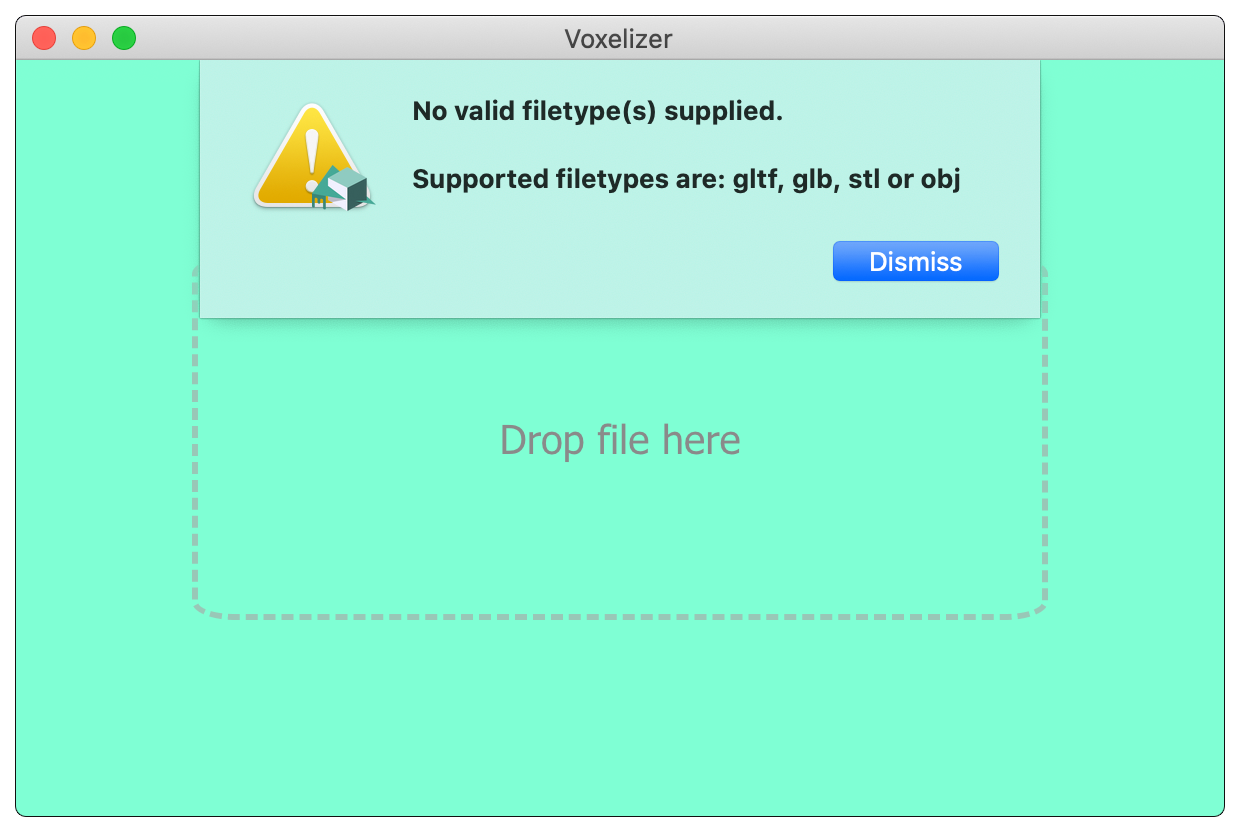
\includegraphics[width=0.9\textwidth]{sections/result/figures/voxelizer-desktop-gui-dnd-file-warning.png}
    \caption{Voxelizer Desktop drag and drop start screen filetype error.}
    \label{fig:voxelizer-desktop-gui-dnd-file-warning}
\end{figure}
\begin{figure}[htp]
    \centering
    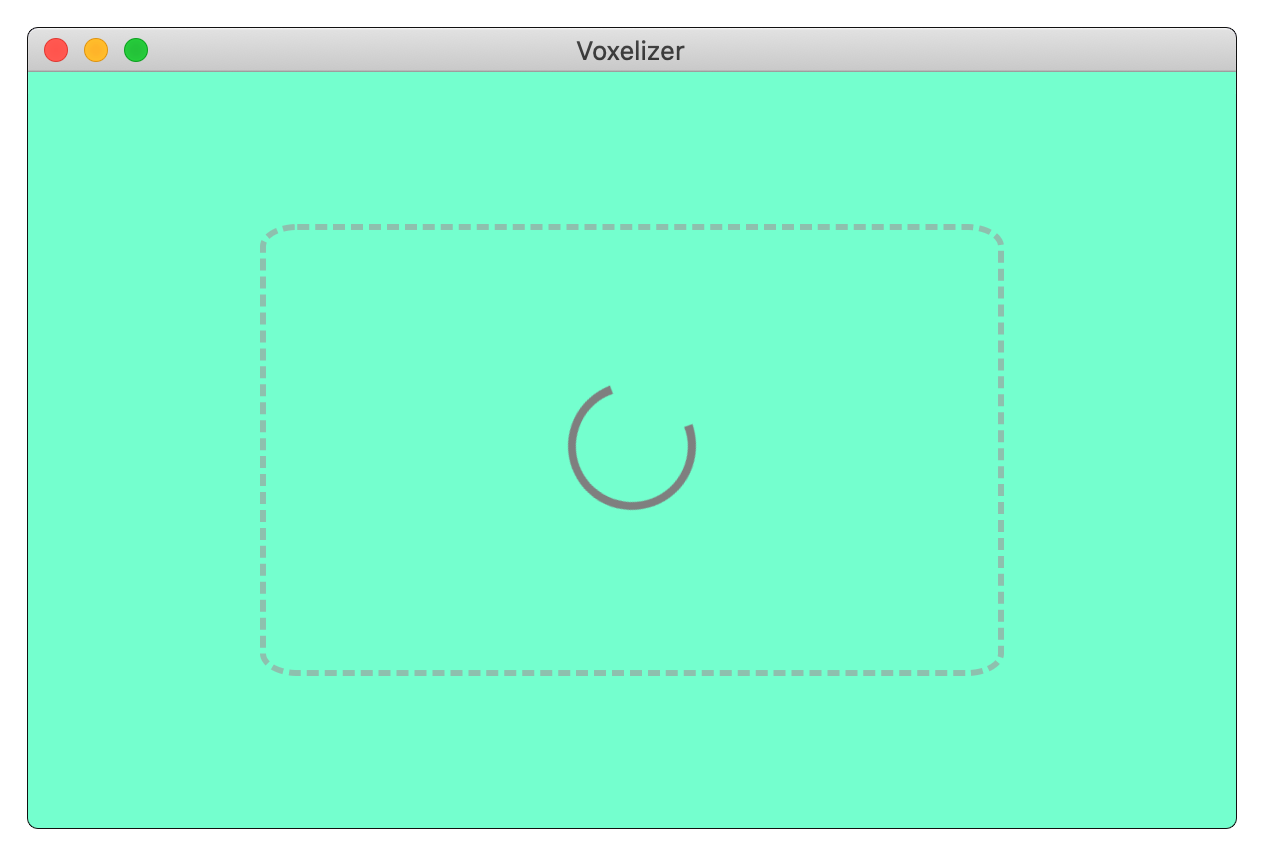
\includegraphics[width=0.9\textwidth]{sections/result/figures/voxelizer-desktop-gui-loading.png}
    \caption{Voxelizer Desktop loading 3D model.}
    \label{fig:voxelizer-desktop-gui-loading}
\end{figure}
\clearpage

When the loading finishes, the user is presented with the main interface. This is shown in Figure~\ref{fig:voxelizer-desktop-gui-main-light}. Here, the loaded 3D model is first presented in an interactive display. Further, at the bottom there are various controls for the voxelization and for exporting.
\begin{figure}[htp]
    \centering
    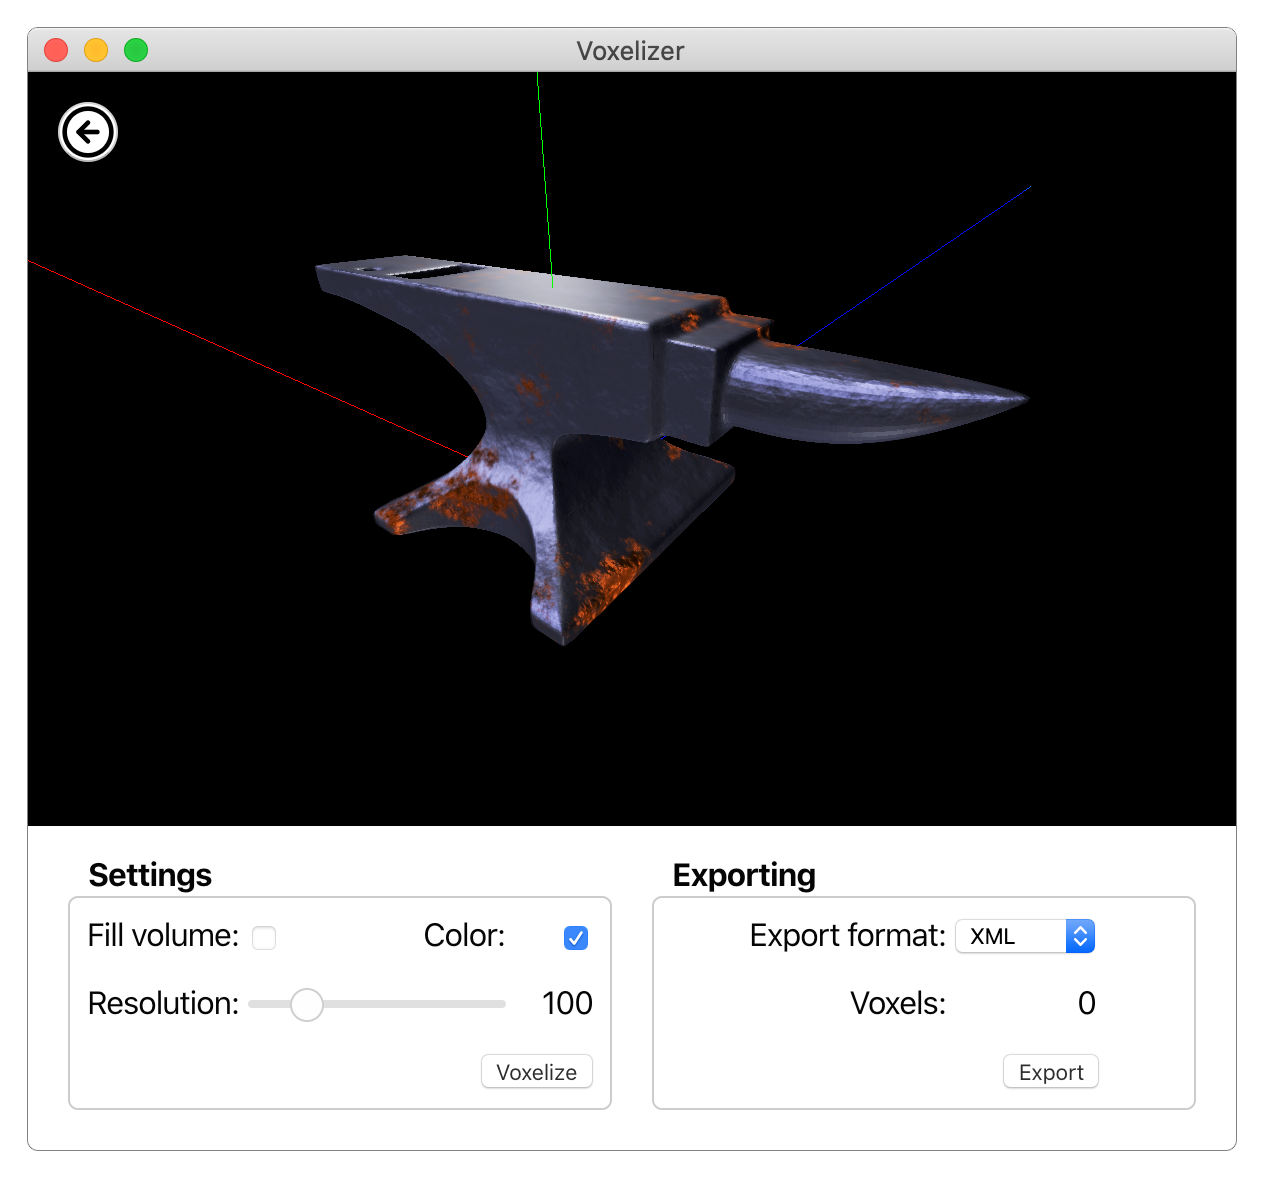
\includegraphics[width=0.9\textwidth]{sections/result/figures/voxelizer-desktop-gui-main-light.png}
    \caption{Voxelizer Desktop main interface.}
    \label{fig:voxelizer-desktop-gui-main-light}
\end{figure}
\clearpage

The application has support for dark mode. Meaning, depending on the system settings, either a light-theme or a dark-theme is selected. The application also has localization support (language). Currently, English and Norwegian Bokmål is available. The selected language will depend on the system settings. Figure~\ref{fig:voxelizer-desktop-gui-main-dark} shows the main interface in dark mode and with a Norwegian interface.
\begin{figure}[htp]
    \centering
    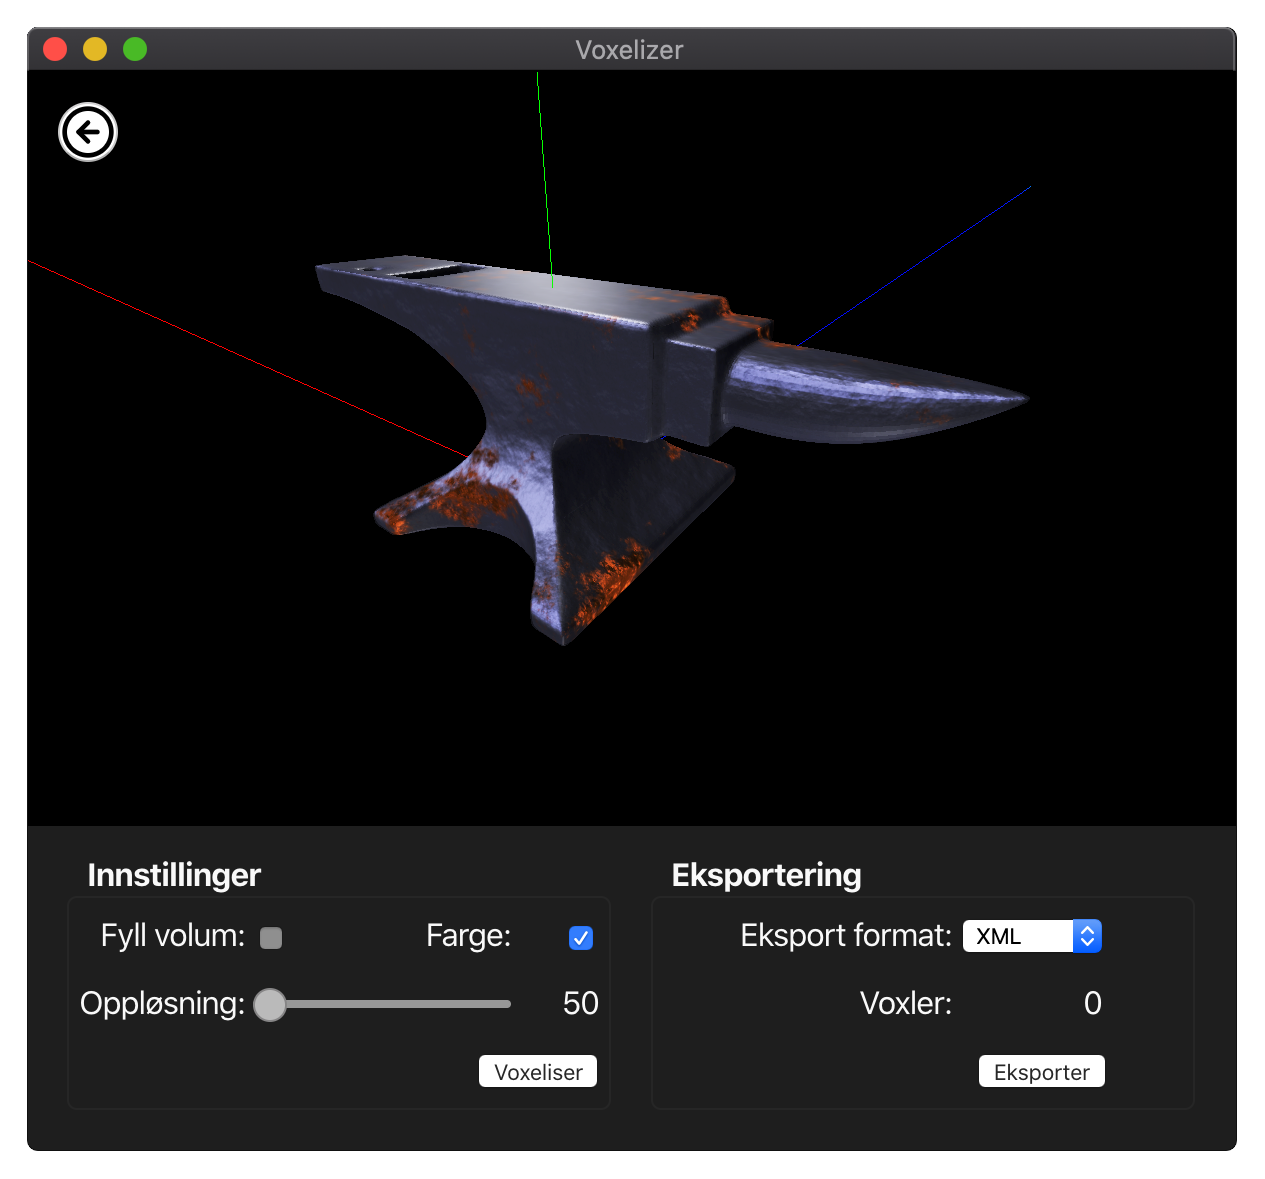
\includegraphics[width=0.9\textwidth]{sections/result/figures/voxelizer-desktop-gui-main-dark.png}
    \caption{Voxelizer Desktop with dark mode and Norwegian language.}
    \label{fig:voxelizer-desktop-gui-main-dark}
\end{figure}
\clearpage

If one tries to export before voxelizing the model, a modal will show a warning message. Figure~\ref{fig:voxelizer-desktop-gui-main-voxel-warning} shows this error message.
\begin{figure}[htp]
    \centering
    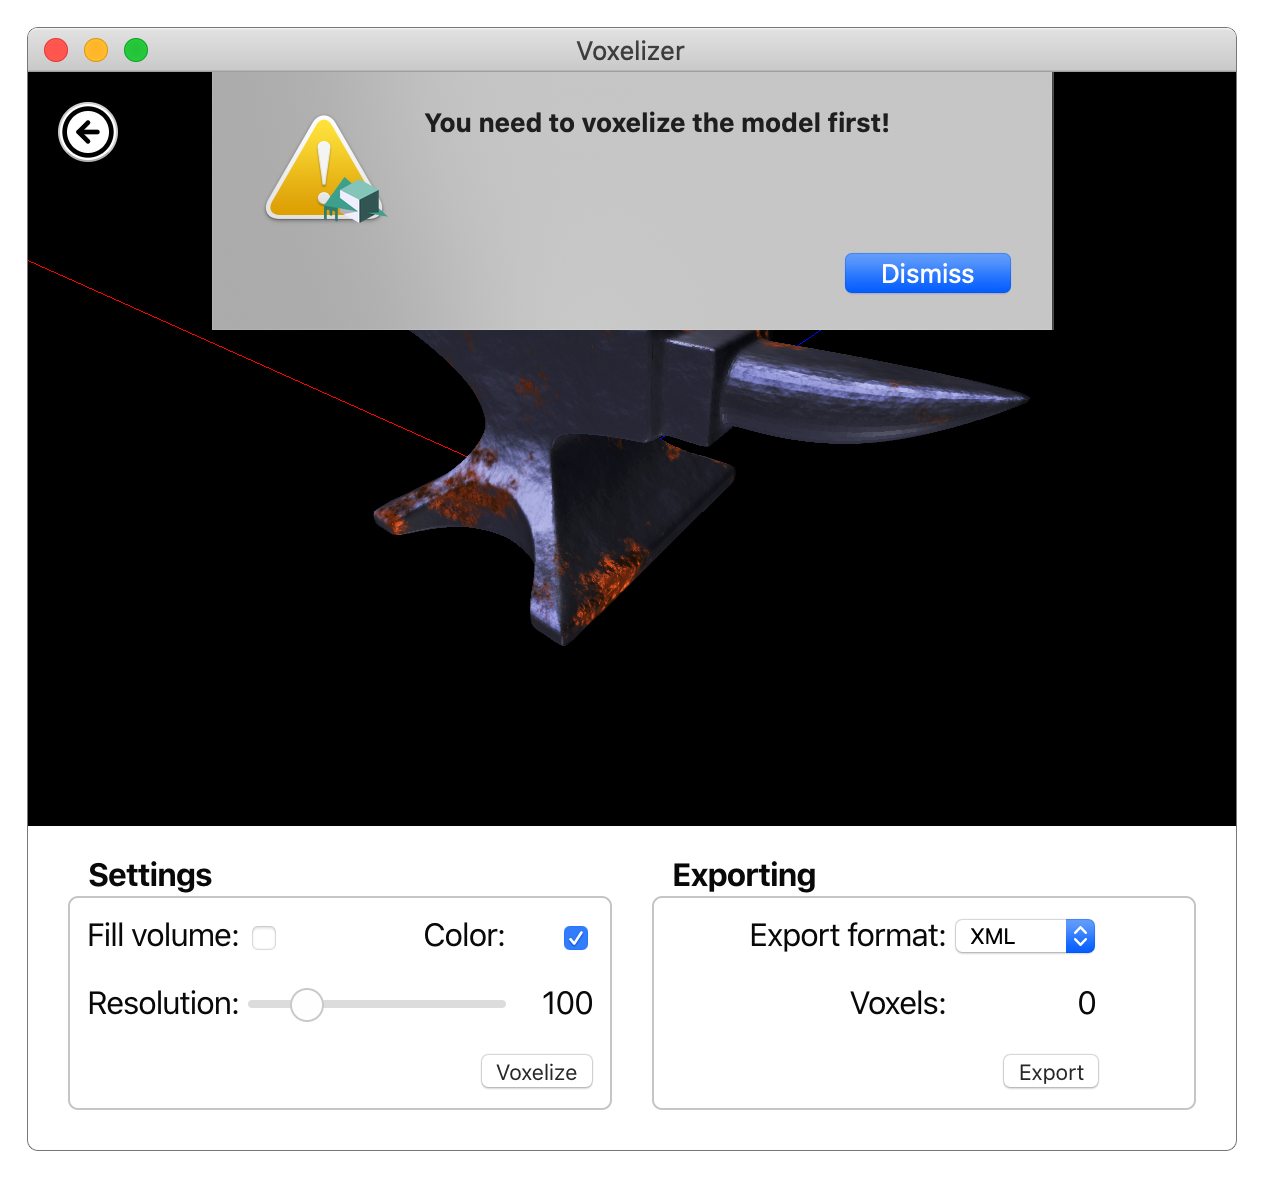
\includegraphics[width=0.9\textwidth]{sections/result/figures/voxelizer-desktop-gui-main-voxel-warning.png}
    \caption{Voxelizer Desktop voxel warning.}
    \label{fig:voxelizer-desktop-gui-main-voxel-warning}
\end{figure}
\clearpage

To actually voxelize the model, the user needs to click on the \textbf{Voxelize} button. This starts the voxelization process. When finished, the result is presented in the 3D graphics window. This can be seen in Figure~\ref{fig:voxelizer-desktop-gui-voxels}
\begin{figure}[htp]
    \centering
    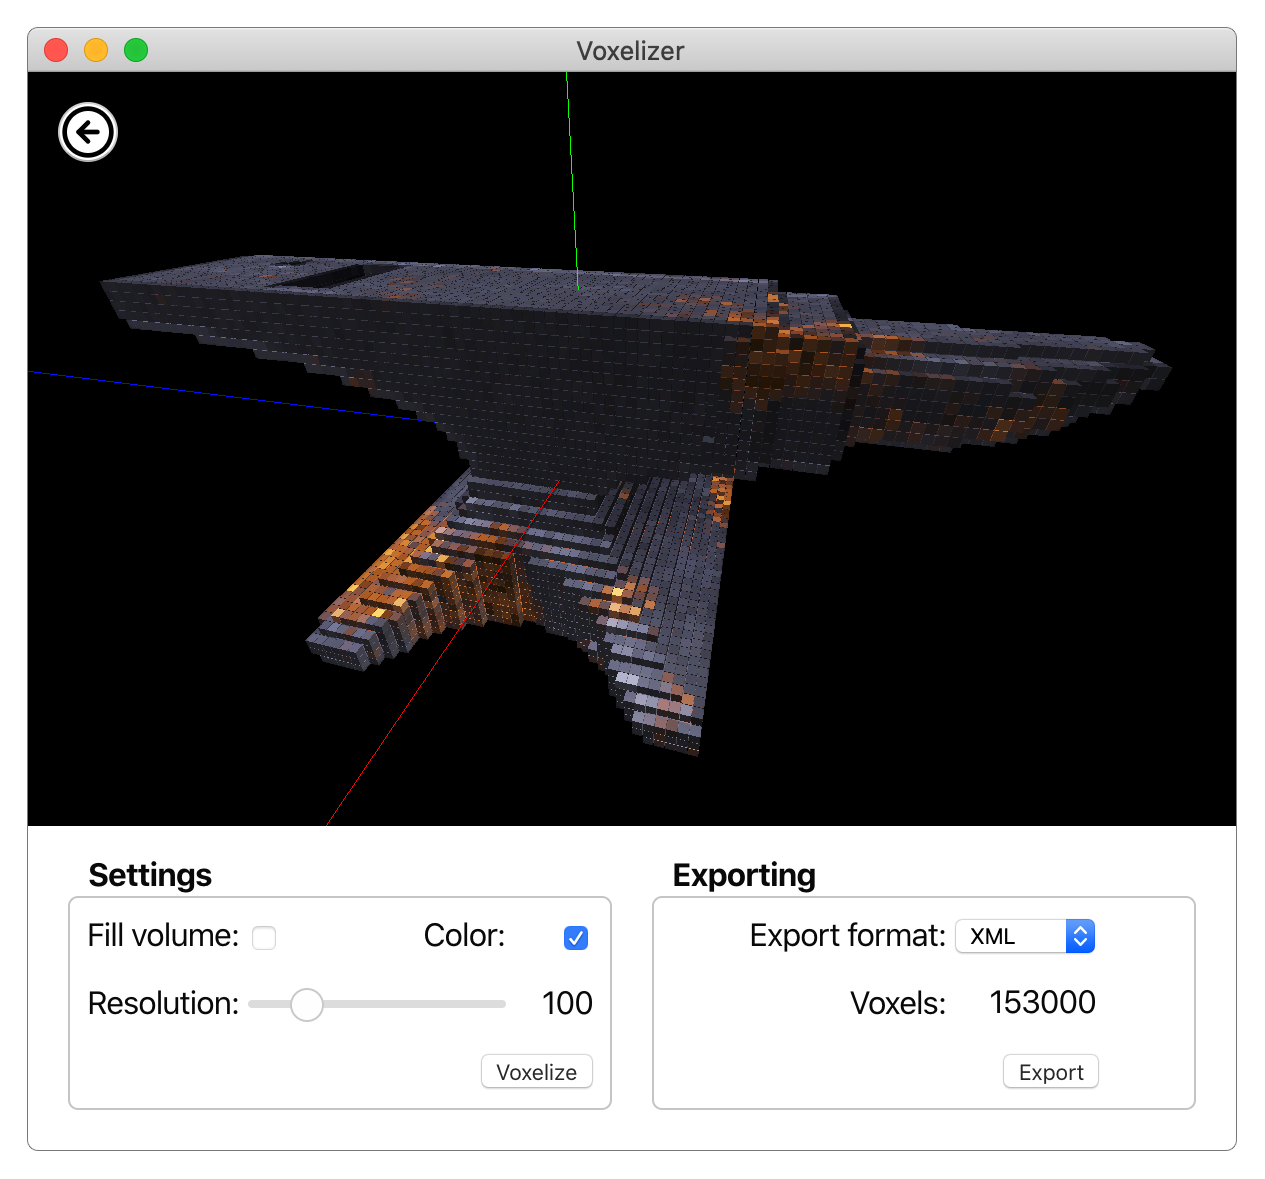
\includegraphics[width=0.9\textwidth]{sections/result/figures/voxelizer-desktop-gui-voxels.png}
    \caption{Voxelizer Desktop displaying voxelized result.}
    \label{fig:voxelizer-desktop-gui-voxels}
\end{figure}
\clearpage

To export and save the voxel data in the selected file format, the user needs to click on the \textbf{Export} button. This opens up the operating system's file system dialog, as can be seen in Figure~\ref{fig:voxelizer-desktop-gui-export}. A file name and location then needs to be provided. When the user clicks on the \textbf{Save} button, the file is saved.
\begin{figure}[htp]
    \centering
    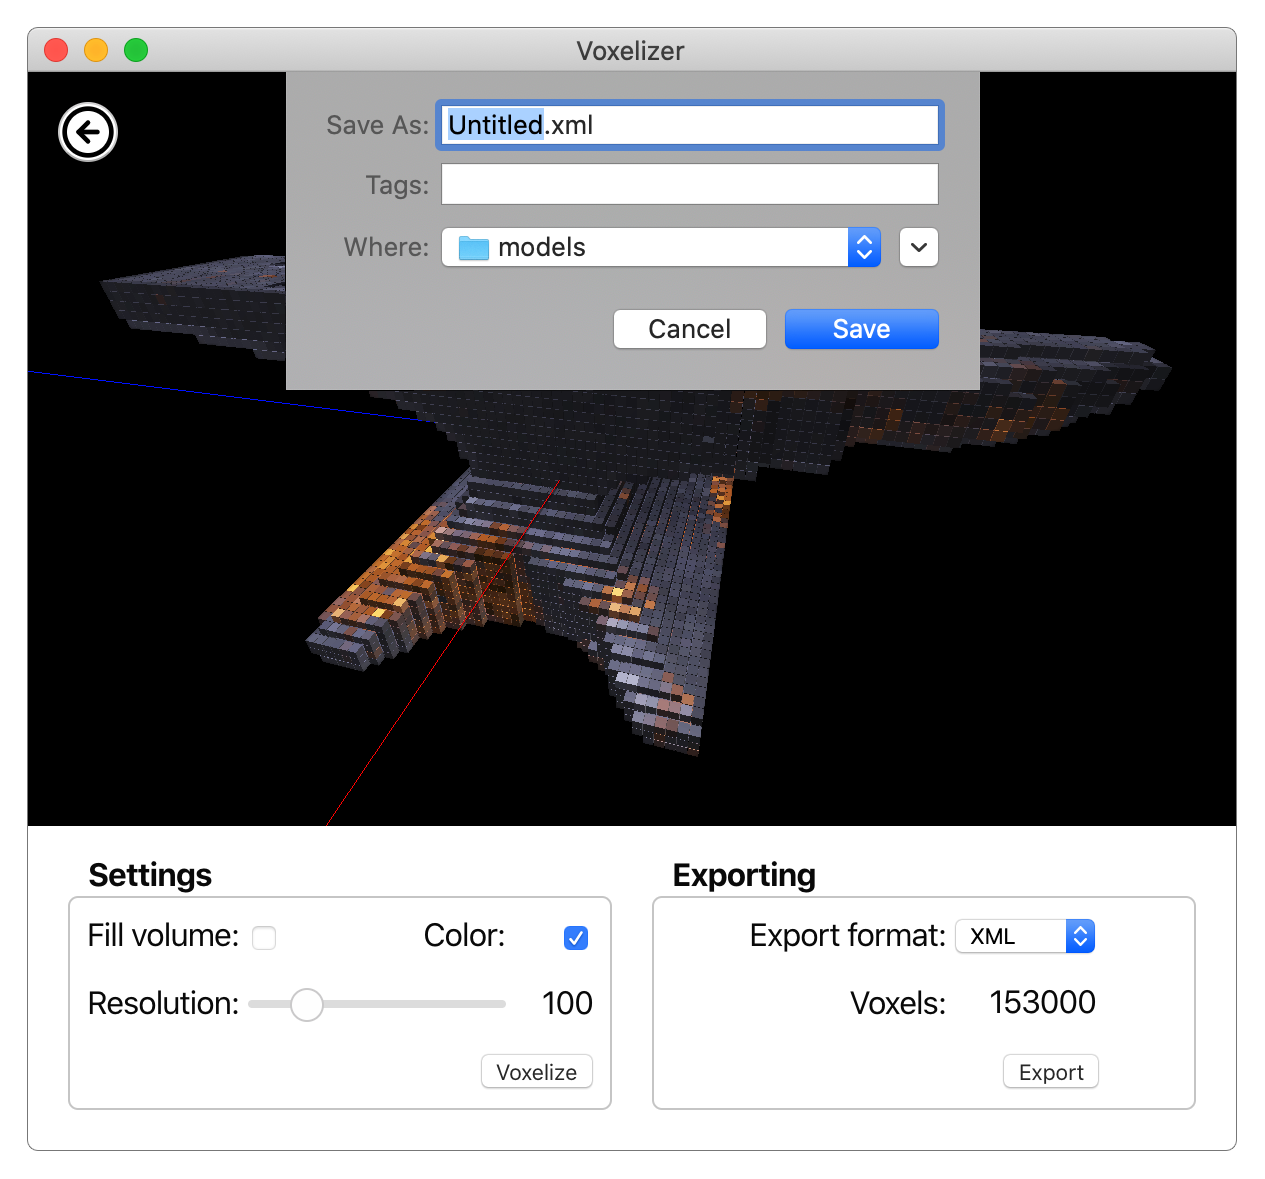
\includegraphics[width=0.9\textwidth]{sections/result/figures/voxelizer-desktop-gui-export.png}
    \caption{Voxelizer Desktop OS file dialog for saving voxel data.}
    \label{fig:voxelizer-desktop-gui-export}
\end{figure}

In order to voxelize a different 3D model, the user can click on the arrow icon in the upper left corner. When the user exits the application, the application state is saved. Among other things, this enables the application window to remember its window location and size.

\section{JSDoc Action}
\label{sec:result-jsdoc-action}
The JSDoc Action makes it easy to automate the process of generating JSDoc documentation. It is a GitHub Action, and is published to the GitHub Marketplace under the name "\href{https://github.com/marketplace/actions/jsdoc-action}{JSDoc Action}". Figure~\ref{fig:jsdoc-action-logo} shows the graphics generated by the GitHub Marketplace for the JSDoc Action. The source code is available at GitHub under "\href{https://github.com/andstor/jsdoc-action}{andstor/jsdoc-action}".
\begin{figure}[htp]
    \centering
    
\includegraphics[width=0.75\textwidth]{sections/result/figures/jsdoc-action-logo.png}
    \caption{Graphics from the GitHub Marketplace for the JSDoc Action.}
    \label{fig:jsdoc-action-logo}
\end{figure}

The action is easy to combine with other deployment actions. This makes it very simple to publish the generated documentation to any hosting service, for example GitHub Pages. The JSDoc Action also supports templates. These are installed with npm, so any package can be used. See the npm documentation for more details on the installation command~\cite{npm-install-docs}.

All that is needed for a minimum base setup is a workflow step like the one defined in Listing~\ref{lst:jsdoc-action-workflowstep}. This will generate documentation for all source files in the "./src" directory, and output the built files to a "./out" directory. Any other GitHub Action might further process this output.
\begin{lstlisting}[language=yaml,caption={Basic JSDoc Action workflow step},label={lst:jsdoc-action-workflowstep}]
- name: Build docs
  uses: andstor/jsdoc-action@v1
  with:
    source_dir: ./src
    recurse: true
    output_dir: ./out
\end{lstlisting}

\subsection{Example usage}
In the following, a complete example to illustrate how easy it is to automate the JSDoc documentation process with the JSDoc Action is provided. This assumes that GitHub is used for hosting the code to generate documentation for.

First, a workflow yaml file needs to be created. This file needs a name, for example \textbf{documentation.yaml}, and has to be uploaded to the default branch in the user's repository, under ".github/workflows/". Then, the actual workflow needs to be defined. Listing~\ref{lst:jsdoc-workflow-deploy-example} provides an example workflow. This workflow is set to only run when code is pushed to the master branch. Ubuntu is then chosen as the platform to run the workflow job on. Several workflow steps are then defined:
\begin{enumerate}
    \item First, the user's code repository is cloned with the help of the Checkout Action by GitHub. This makes the user's source code available to subsequent steps. 
    \item Second, the JSDoc Action is used for generating the actual JSDoc documentation files. Lines 15-19 defines several input options to the JSDoc Action. The source directory is set to "./src". The output directory is set to "./out". A path to a JSDoc configuration file in the user's repository is then specified. In order to freshen up the plain JSDoc theme, the minami template is used. This is the name of the package on npm. Finally, the README.md file in the user's repository is used as frontpage. 
    \item Third, the GitHub Pages action is used for deploying the generated documentation files to GitHub Pages. It needs two input configurations. One is a deployment key. See the documentation for the GitHub Pages action for how to set up this. The other is a directory where the files to publish resides. This is set to the the JSDoc Action's output directory, "./out".
\end{enumerate}
When the workflow file is finished and saved to the correct place, the repository will feature automatic JSDoc documentation generation.

\clearpage
\lstinputlisting[language=yaml,style=numbers,label={lst:jsdoc-workflow-deploy-example},caption={Example documentation workflow file}]{sections/result/code/documentation-workflow.yaml}

\section{file-existence-action}
The File Existence action is a GitHub Action. The action is published to the GitHub Marketplace by the name "\href{https://github.com/marketplace/actions/file-existence}{File Existence}", and the source code is available at GitHub under "\href{https://github.com/andstor/file-existence-action}{andstor/file-existence-action}".

The action is able to check if one or more files exists during a workflow run. The user just supplies the paths as inputs to the action. The action then produces a boolean output variable which is available to the subsequent workflow steps. If any files are missing, the output is set to false. Otherwise, true. It is also possible to make the action trigger an error if one or more files are missing. This will effectively cancel the entire workflow.

\section{file-reader-action}
The File Reader action is a GitHub Action. The action is published to the GitHub Marketplace by the name "\href{https://github.com/marketplace/actions/file-reader}{File Reader}", and the source code is available at GitHub under "\href{https://github.com/andstor/file-reader-action}{andstor/file-reader-action}".

By providing a path as input to the action, the action is simply able to read the contents of a file during a workflow run. The action produces an output variable with the contents of the file. This variable will be available to the subsequent workflow steps.

\section{Automation}
\label{sec:result-automation}
Several automation systems are implemented for the various projects. This makes the maintenance of the projects very easy. All JavaScript package building and publishing is fully automated. Automatic JSDoc generation and publishing is also set up. Further, maintenance tasks for the GitHub actions are automated. See Section~\ref{sec:method-automation} for a walkthrough of how the automations systems work, and what they do in details. For the GitHub Actions, automatic updating of version tags are implemented, according to the GitHub guidelines. For the JavaScript packages, the following tasks are automated:
\begin{itemize}
    \item Building
    \item Testing
    \item Code coverage generation, and uploading to Coveralls.io
    \item Security analysis with LGTM by Semmle
    \item JavaScript JSDoc documentation generation with the JSDoc Action
    \item Publishing of JavaScript package to the npm registry
\end{itemize}
Figure~\ref{fig:automation-pull-request} shows how some of these automated task (defined in Workflows) are run on GitHub's CI/CD system. Here, one can see all the checks are passed. Also, an alert is triggered by the security analysis by LGTM, stating that three new alerts are introduced in the code.
\begin{figure}[htp]
    \centering
    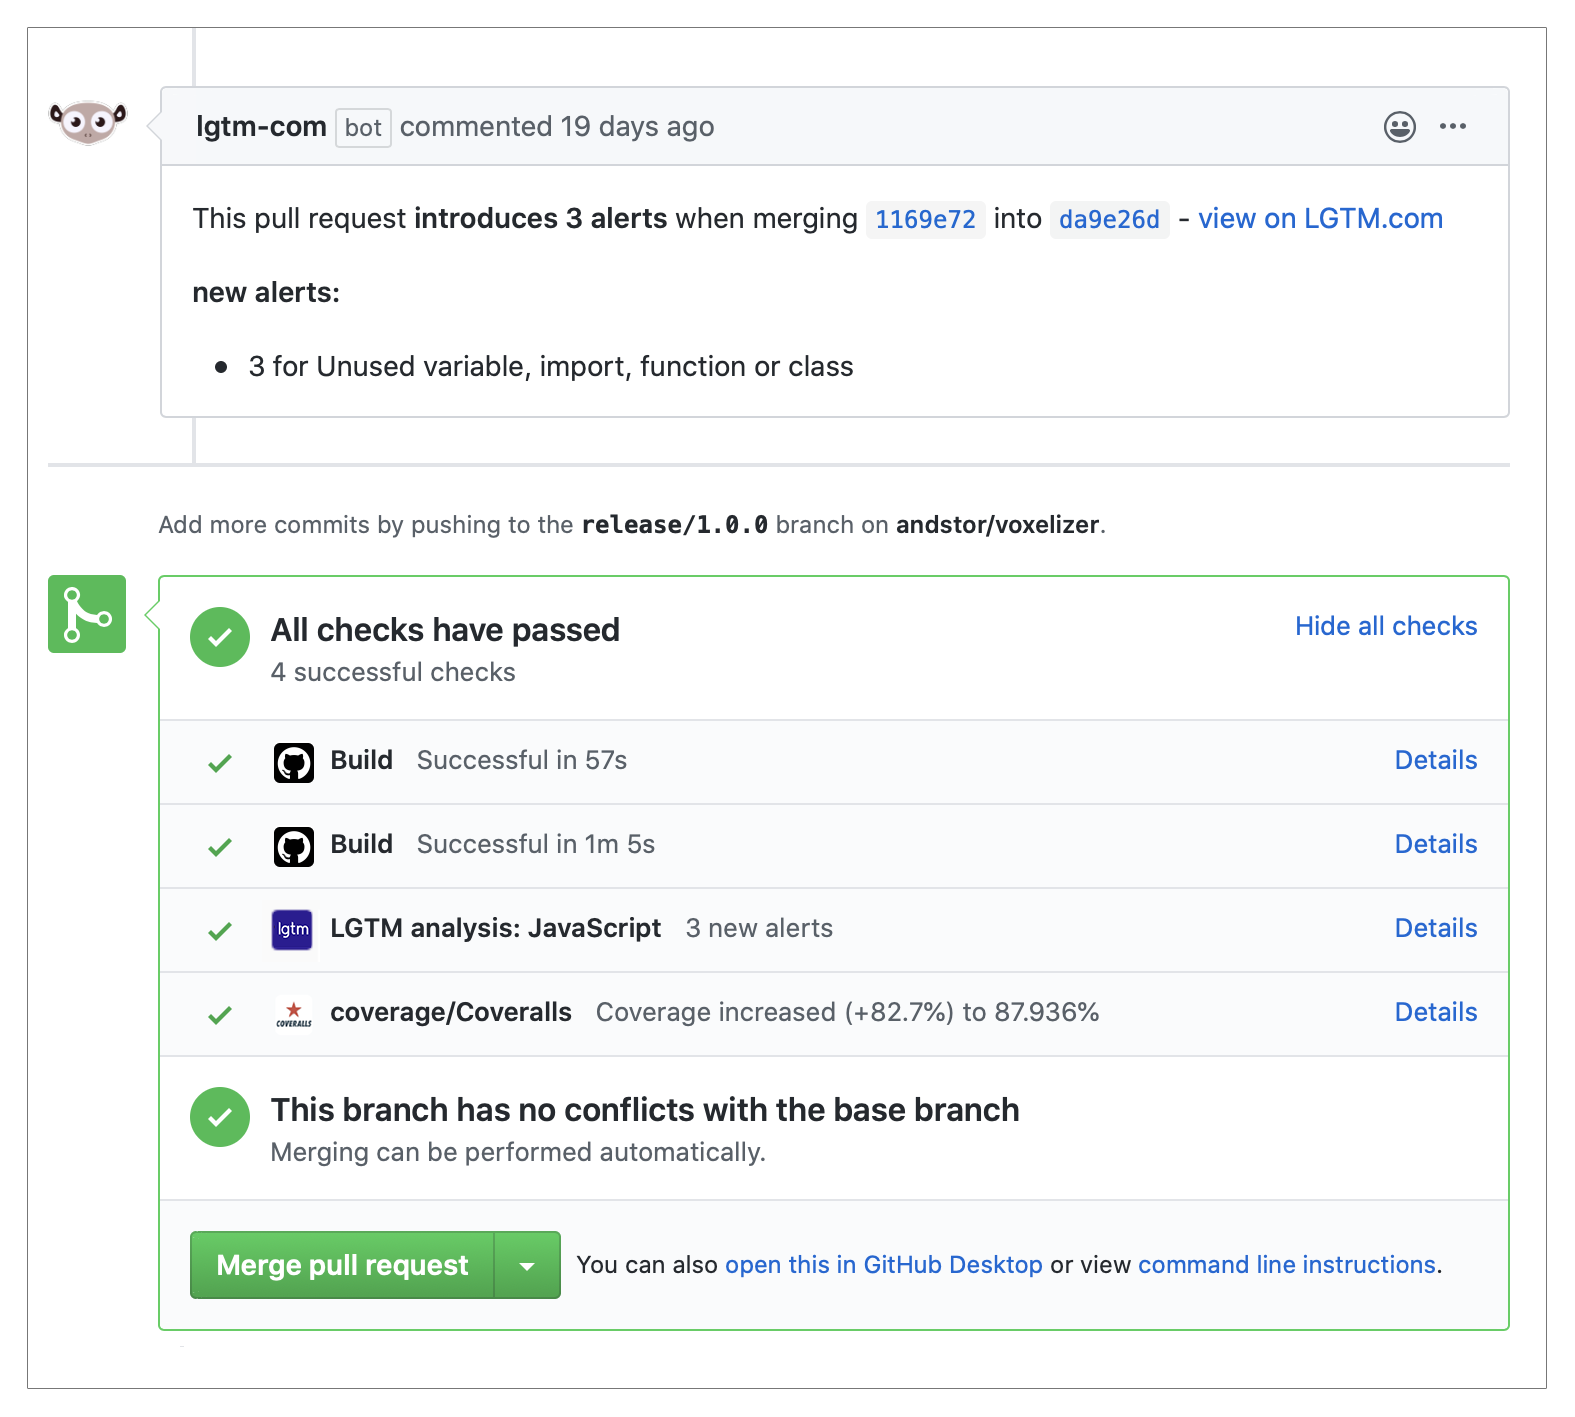
\includegraphics[width=\textwidth]{sections/result/figures/automation-pull-request.png}
    \caption{Screenshot of automation checks for a pull request on GitHub.}
    \label{fig:automation-pull-request}
\end{figure}

\section{Popularity and achievements}
\label{sec:result-popularity-and-achievements}
Several of the projects has already gained interest by the public. GitHub users are able to star a repository. This is one of the main measurements available for how popular a repository is. Several of the repositories created in connection with this thesis have received numerous of stars already, and is used by several people. Table~\ref{tab:statistics-github-repos} shows how many stars the different repositories have, as of May 17th, 2020 \footnote{The statistics also include personal staring and usage.}.
\begin{table}[ht]
    \newcolumntype{Y}{>{\centering\arraybackslash}X}
    \def\arraystretch{1.5}
    \centering
    \medskip
    \caption{Repositories statistics as of May 17th, 2020.}
    \label{tab:statistics-github-repos}
    \begin{tabularx}{0.5\textwidth}{|Y|c|c|}
        \hline
        \textbf{Repository} & \textbf{Stars} &  \textbf{Used by}\\
        \hline
        jsdoc-action & 13 & 22\\
        file-existence-action & 6 & 17\\
        voxelizer & 4 & 3\\
        three-voxel-loader & 4 & 1\\
        file-reader-action & 1 & 5\\
        binvox & 1 & 2\\
        voxelizer-desktop & 1 & 0\\
        \hline
    \end{tabularx}
\end{table}

Another achievement is the inclusion of a link to the JSDoc Action in the \href{https://github.com/jsdoc/jsdoc/blob/master/README.md}{README.md} file of the original JSDoc repository. As of May 17th, 2020 the JSDoc repository has 10.6 thousand stars and is used in by more than 39.300 repositories. This gives the action a lot of marketing. The approved pull request is number \href{https://github.com/jsdoc/jsdoc/pull/1745}{\#1745}. 
Figure~\ref{fig:jsdoc-link-readme} shows a screenshot of the \textbf{Templates and tools} section of the README.md file. The link to the JSDoc Action is located at the bottom of the \textbf{Build tools} subsection, marked in red.
Figure~\ref{fig:comment-hegemonic} shows the response to the approved pull request from the lead maintainer Jeff Williams (\href{https://github.com/hegemonic}{hegemonic}) of JSDoc.
\begin{figure}[htp]
    \centering
    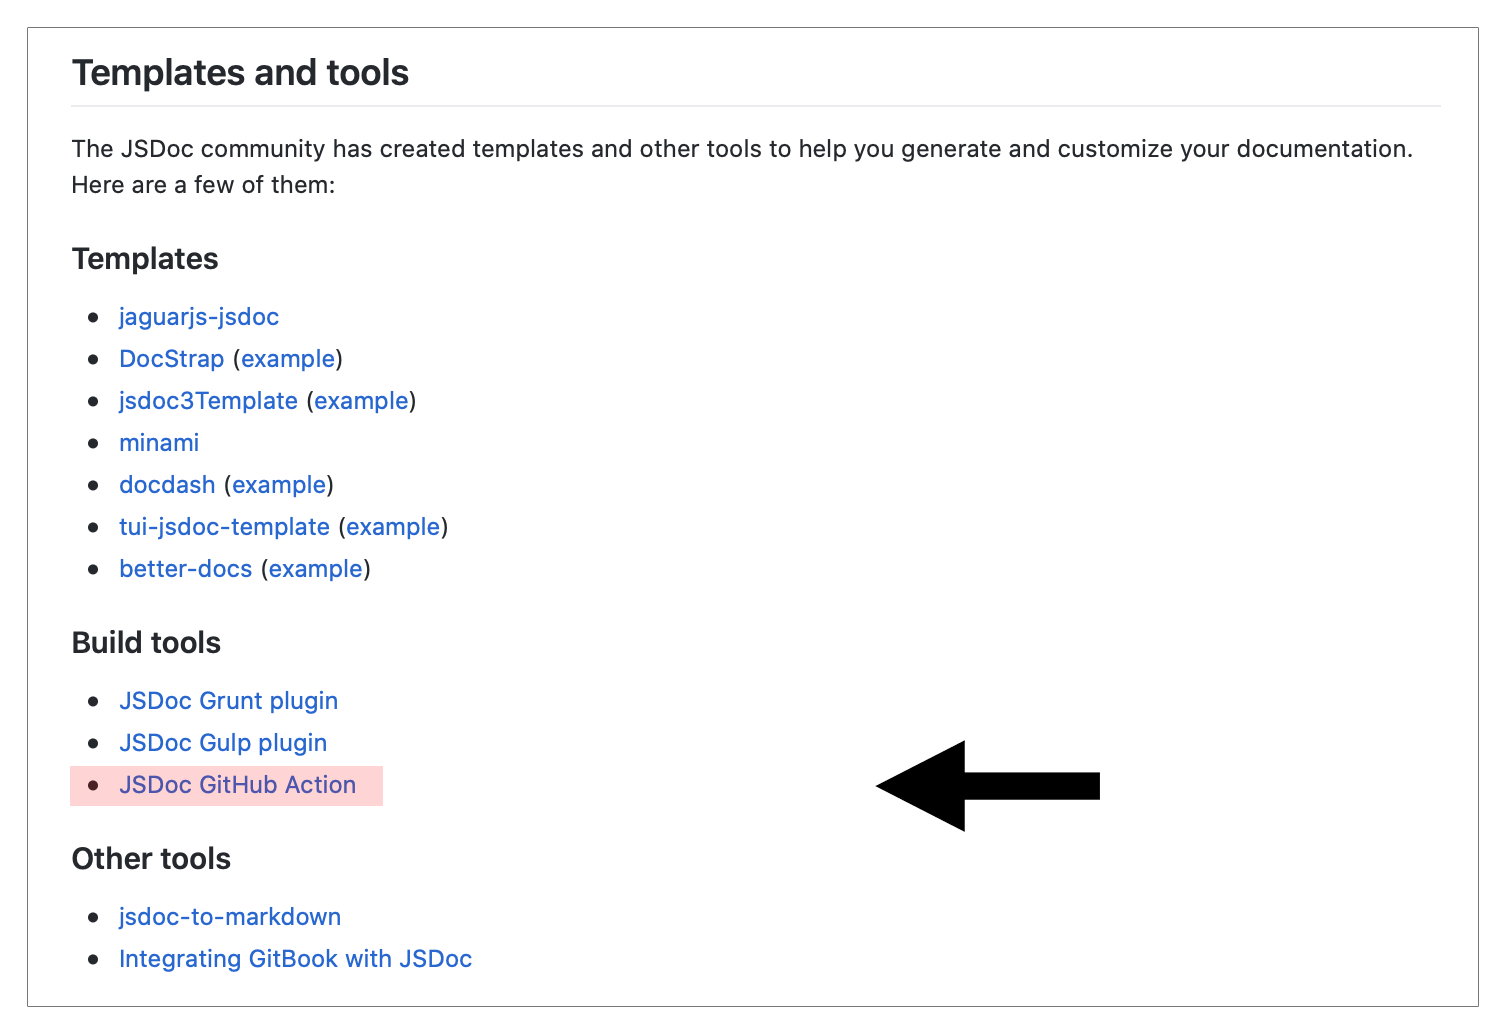
\includegraphics[width=\textwidth]{sections/result/figures/jsdoc-readme.png}
    \caption{Screenshot of JSDoc README.md file.}
    \label{fig:jsdoc-link-readme}
\end{figure}
\begin{figure}[htp]
    \centering
    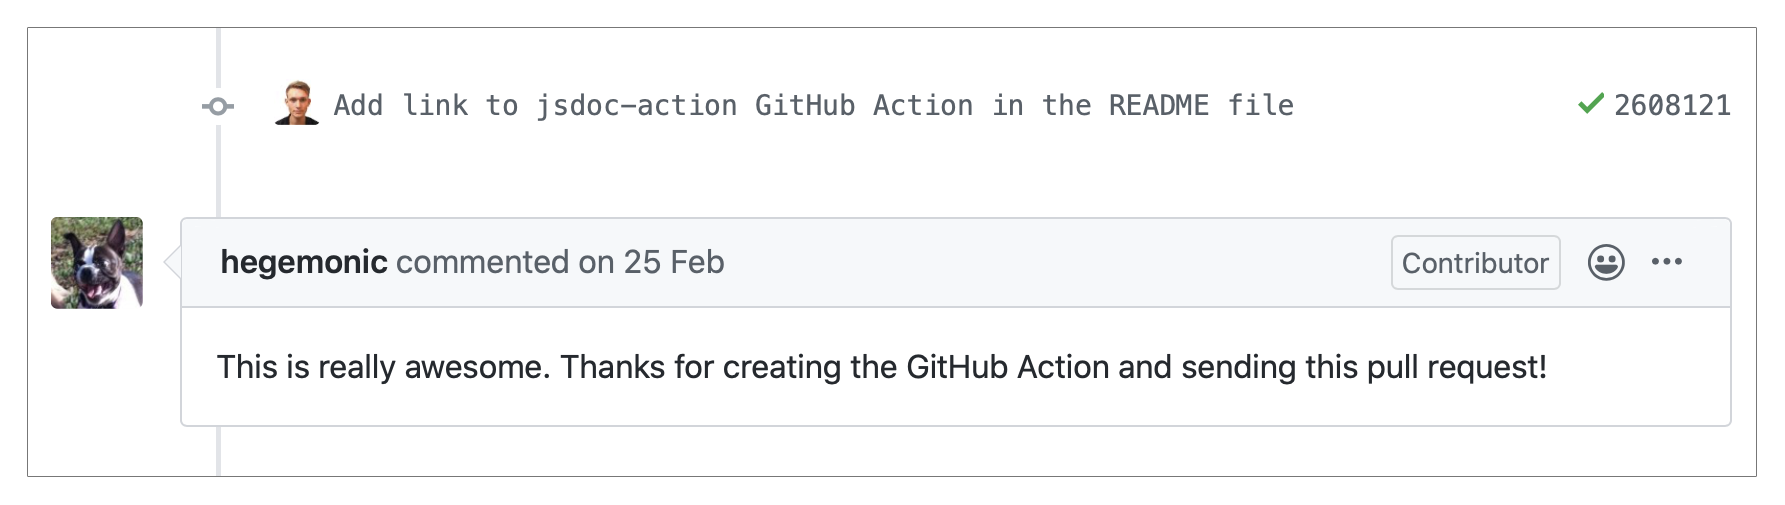
\includegraphics[width=\textwidth]{sections/result/figures/jsdoc-action-pull-request-approval-jsdoc.png}
    \caption{Screenshot of response from JSDoc lead maintainer.}
    \label{fig:comment-hegemonic}
\end{figure}
